\documentclass[11pt,a4paper]{article}
\usepackage[spanish]{babel}
\usepackage[T1]{fontenc}
\usepackage[utf8]{inputenc}
\usepackage[margin=2.3cm]{geometry}
\usepackage{amsmath,amssymb,booktabs,array}
\usepackage{hyperref}
\hypersetup{hidelinks}
\usepackage{graphicx}
\usepackage{placeins}
\newcommand{\pct}{\text{\char37}}
\setlength{\parskip}{0.35em}
\renewcommand{\arraystretch}{1.15}
\title{Sensibilidad del aerogenerador:\\ resultados, mecanismos e interpretación}
\author{Documento de apoyo para la discusión con el asesor de tesis}
\date{Morris y rejilla de octubre; comparación sísmica y eólica del 20 de octubre de 2026}
\begin{document}
\maketitle

\section{Qué se puede concluir del estudio}
La pregunta estudiada es cómo cambian las frecuencias del modelo existente al modificar propiedades de las palas y velocidad del rotor. La respuesta depende del grupo modal. Entre los \emph{tres factores comparados}, la masa e inercia de palas tienen la mayor influencia media en las respuestas 3, 4+5, 8+9 y 10+11; la velocidad del rotor tiene la mayor influencia media en 6+7. Esta clasificación se refiere a un dominio exploratorio de factores entre 0.90 y 1.10.

Se completaron cuarenta trayectorias Morris: 160 evaluaciones del diseño y diez controles numéricos, todas convergidas. El diseño visitó 58 combinaciones diferentes; sus repeticiones se conservaron. Se aceptaron catorce indicadores de influencia media de frecuencia. Su cambio entre veinte y cuarenta trayectorias fue menor de 1\pct. Se aceptaron dos indicadores de dispersión, asociados a masa y rigidez en 10+11. Estas observaciones constituyen evidencia de sensibilidad del modelo numérico; no son una validación experimental ni una probabilidad de respuesta.

Una forma útil de presentar la contribución es: \emph{se obtuvo un cribado de influencia por grupo modal, con seguimiento de formas, actualización del equilibrio y filtros explícitos de ruido y estabilización}. El aporte científico incluye los signos opuestos del efecto del giro, la compensación parcial masa--rigidez y la identificación de respuestas cuya sensibilidad aún no puede resolverse.


El 14 de octubre se completó la rejilla de 64 combinaciones reutilizando 58 puntos y resolviendo seis faltantes. Se añadieron tres controles numéricos. Los nueve casos nuevos convergieron, sin cambios de rangos ni formulación. El contraste masa--rigidez de 10+11 supera la envolvente empírica en las cuatro velocidades examinadas.

\section{Qué se varió y qué representa el modelo}
Se denotan los factores por $\xi_\rho$ (masa e inercias de palas), $\xi_K$ (rigideces seccionales de palas) y $\xi_\Omega$ (velocidad del rotor). Su nominal es uno. El subíndice $\rho$ expresa un escalamiento compatible con cambio de densidad a geometría fija; no identifica una densidad experimental única de las palas.

\begin{center}\small
\begin{tabular}{p{2cm}p{7.1cm}p{3.7cm}}
\toprule Factor & Cambio consistente & Intervalo aprobado \\ \midrule
$\xi_\rho$ & Masa por longitud e inercias seccionales de las tres palas, con geometría y centroides fijos. & 0.90--1.10 \\
$\xi_K$ & Rigideces axial, de cortante, torsional y de flexión de las palas, escaladas conjuntamente. & 0.90--1.10 \\
$\xi_\Omega$ & Velocidad prescrita alrededor del eje del rotor, constante en cada caso. & 10.8--13.2 rpm \\
\bottomrule
\end{tabular}
\end{center}
Los rangos son escenarios aprobados, no límites de fabricación medidos. Los restantes parámetros conservan sus valores en esta campaña. Por ello, la clasificación global no compara exhaustivamente palas, torre, cimentación y conexiones.

\begin{figure}[htbp]
\centering
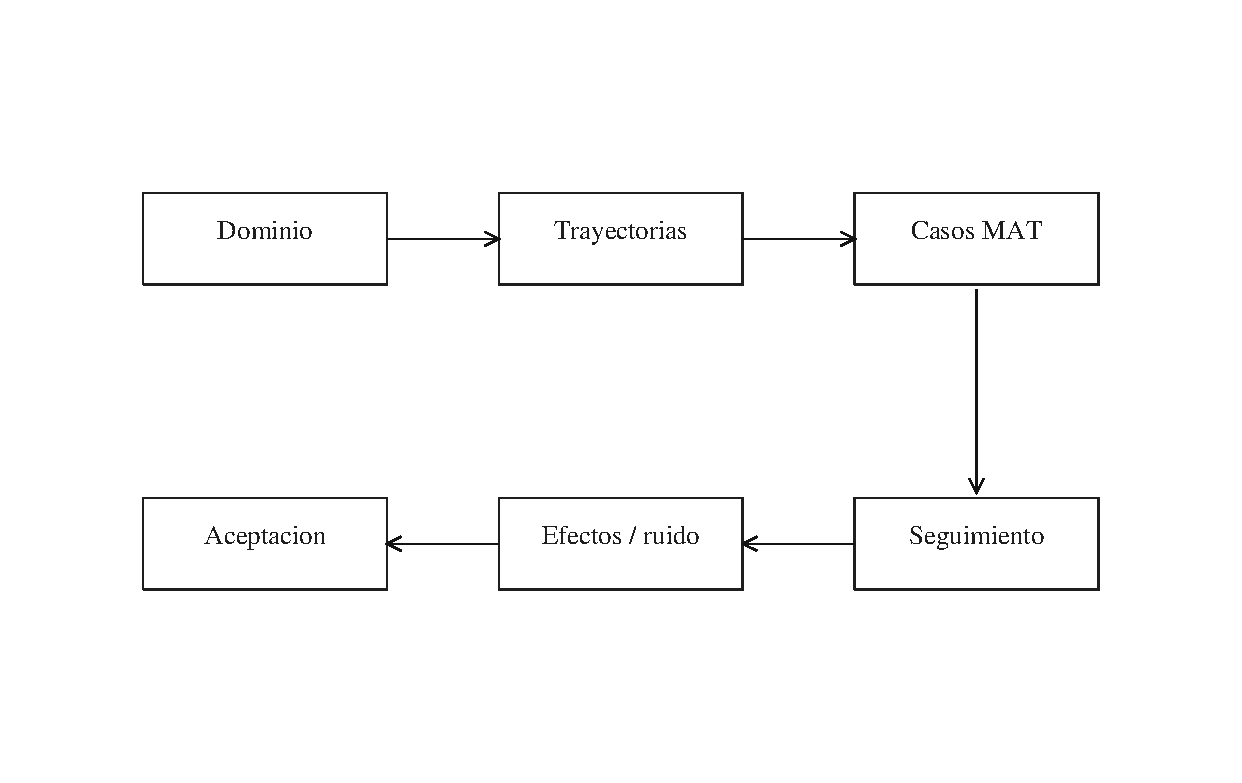
\includegraphics[width=.96\linewidth,height=.40\textheight,keepaspectratio]{figures/tecplot/morris_proceso.pdf}
\caption{Flujo del posprocesamiento de sensibilidad: dominio exploratorio, trayectorias, casos almacenados, seguimiento, efectos frente al ruido y aceptación. Cada caso es un equilibrio independiente a azimut congelado; la sensibilidad total incluye el cambio del equilibrio y de los operadores. El giro se prescribe alrededor del eje 129--130, sin guiñada nominal.}\label{fig:proceso}
\end{figure}

\section{Cómo leer las frecuencias y los grupos}
Sea $\boldsymbol q$ el vector de coordenadas perturbadas alrededor del equilibrio y $t$ el tiempo. Los operadores efectivos de masa, velocidad y tangente se denotan por $\mathsf M$, $\mathsf D$ y $\mathsf K$. La parte homogénea de la linealización congelada se escribe
\begin{equation}
\mathsf M\ddot{\boldsymbol q}+\mathsf D\dot{\boldsymbol q}+\mathsf K\boldsymbol q=\boldsymbol 0.
\end{equation}
La matriz $\mathsf D$ reúne amortiguamiento, efectos giroscópicos y transporte; sus términos no representan todos disipación material. La tangente $\mathsf K$ incluye las contribuciones implementadas del equilibrio y del giro, con las transformaciones cinemáticas correspondientes.

Sean $\lambda$ una raíz compleja y $\boldsymbol\phi$ su forma modal. Con $\boldsymbol q\propto\boldsymbol\phi\exp(\lambda t)$ se obtiene el problema cuadrático
\begin{equation}
[\lambda^2\mathsf M+\lambda\mathsf D+\mathsf K]\boldsymbol\phi=\boldsymbol 0.
\end{equation}
Se definen frecuencia amortiguada $f_d=|\operatorname{Im}\lambda|/(2\pi)$ [Hz], crecimiento $\gamma=\operatorname{Re}\lambda$ [s$^{-1}$] y razón de amortiguamiento $\zeta=-\operatorname{Re}\lambda/|\lambda|$. La frecuencia mide oscilaciones por segundo; el crecimiento mide evolución de la envolvente. Una frecuencia que aumenta no implica, por sí sola, mayor estabilidad.

Las etiquetas 6+7 o 10+11 identifican conjuntos de ramas de la referencia, no posiciones que se vuelvan a ordenar por frecuencia en cada caso. Se correlacionan formas complejas en el espacio físico con la masa nominal y se comprueban subespacios cuando hay raíces próximas. La respuesta de un grupo es la \emph{media de las frecuencias de sus ramas}; no constituye una nueva forma modal individual. Las ramas 4 y 5 se agruparon por su proximidad en parte del dominio ampliado. La rama 12 toca la frontera del conjunto seguido y se excluye de los estimadores; sus vecinos del espectro calculado impiden tratarla como grupo cerrado.

\begin{center}\small
\begin{tabular}{lrlp{3cm}}
\toprule Respuesta & $f_{d,0}$ [Hz] & Mayor influencia media & Signo aceptado del giro \\ \midrule
3 & 0.231 & Masa/inercia & $-$ \\
4+5 & 0.409 & Masa/inercia & No resuelto \\
6+7 & 0.587 & Velocidad & $+$ \\
8+9 & 0.844 & Masa/inercia & $+$ \\
10+11 & 1.225 & Masa/inercia & $+$ \\

\bottomrule
\end{tabular}
\end{center}
Aquí $f_{d,0}$ es la frecuencia nominal individual o media del grupo. El giro tiene efecto positivo en tres grupos y negativo en la rama 3. Su efecto en 4+5 permanece no resuelto frente al ruido. Una ausencia de aceptación no significa ausencia de influencia física.

\section{Cómo funciona Morris en este estudio}
Sea $x_i\in[0,1]$ la coordenada normalizada del factor $i$. Se aplica $\xi_i=\ell_i+(u_i-\ell_i)x_i$, donde los límites son $\ell_i=0.90$ y $u_i=1.10$. Se generan trayectorias aleatorias sobre cuatro niveles, con semilla 6706 y paso firmado $\Delta x_i$ de magnitud $2/3$ \cite{morris1991}. Cada segmento cambia un factor y conserva los otros dos. A lo largo de cuarenta trayectorias, ese cambio se observa en diferentes combinaciones del dominio.

\begin{figure}[htbp]
\centering
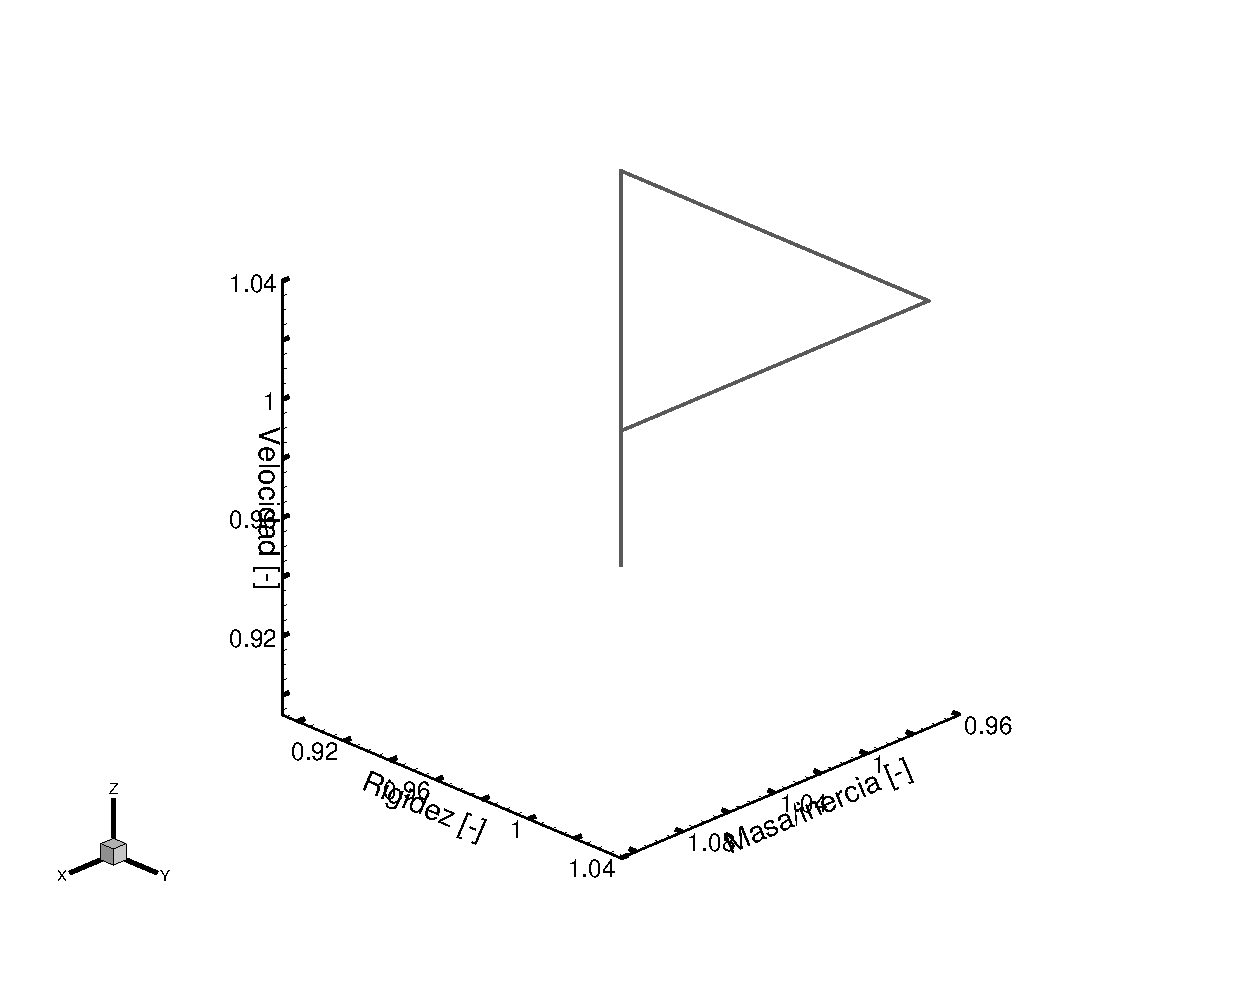
\includegraphics[width=.96\linewidth,height=.40\textheight,keepaspectratio]{figures/tecplot/morris_trayectoria.pdf}
\caption{Primera trayectoria ejecutada en los tres factores del diseño. Cada arista modifica un solo factor. Los segmentos unen casos almacenados y no describen una evolución temporal del rotor.}\label{fig:trayectoria}
\end{figure}
\begin{figure}[htbp]\centering
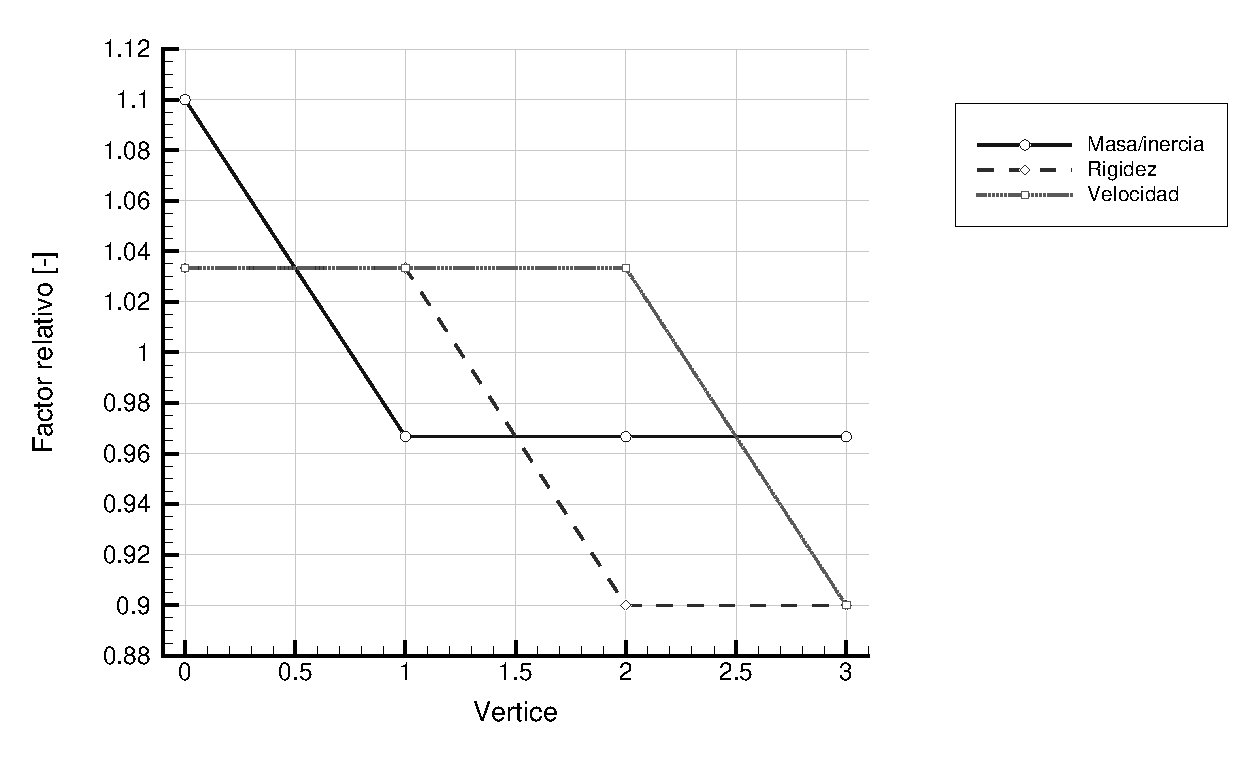
\includegraphics[width=.96\linewidth,height=.40\textheight,keepaspectratio]{figures/tecplot/morris_trayectoria_factores.pdf}
\caption{Factores por vértice de la primera trayectoria, en su orden de evaluación. Los símbolos identifican masa/inercia de palas, rigidez y velocidad. El eje horizontal indica vértices del diseño, no tiempo físico.}\label{fig:trayectoria-factores}\end{figure}

El tamaño del paso del factor es $|\Delta\xi_i|=0.20(2/3)=0.13333$. Aunque los puntos están dentro de $\pm10\pct$ respecto del nominal, cada secante atraviesa 13.333\pct\ del factor nominal. Esta es una razón para distinguir un efecto elemental de una derivada infinitesimal.

Sea $y$ una respuesta escalar y $s_y$ su escala nominal fija. Para frecuencia se usa $s_y=f_{d,0}$; para crecimiento, la media nominal de $|\lambda|$; para amortiguamiento, $\max(|\zeta_0|,0.01)$. El efecto elemental de la trayectoria $j$ es
\begin{equation}
EE_i^{(j)}=\frac{y_{\rm fin}^{(j)}-y_{\rm inicio}^{(j)}}{\Delta x_i^{(j)}s_y}.
\end{equation}
El signo del paso se conserva. Por ejemplo, en la primera arista del grupo 10+11 se \emph{reduce} $\xi_\rho$ de 1.10 a 0.9667 y la frecuencia \emph{aumenta} de 1.203767 a 1.263304 Hz:
\begin{equation}
EE_\rho^{(1)}=\frac{1.263304-1.203767}{(-2/3)(1.225430)}\simeq-0.07288.
\end{equation}
Su signo negativo describe la disminución de frecuencia al \emph{aumentar} masa/inercia. Este ejemplo proviene de casos almacenados; no es una simulación adicional.

Para $r$ trayectorias se calculan
\begin{align}
\mu_i&=\frac{1}{r}\sum_{j=1}^r EE_i^{(j)},&
\mu_i^*&=\frac{1}{r}\sum_{j=1}^r |EE_i^{(j)}|,\\
\sigma_i&=\left[\frac{1}{r-1}\sum_{j=1}^r(EE_i^{(j)}-\mu_i)^2\right]^{1/2}.
\end{align}
$\mu_i$ da dirección media, $\mu_i^*$ magnitud media y $\sigma_i$ dispersión de los efectos entre posiciones del dominio. No son índices de Sobol ni porcentajes máximos de respuesta. No se interpreta el muestreo como una distribución física de incertidumbre. Un efecto inválido impide calcular el estimador correspondiente; no se eliminan aristas selectivamente para obtener una clasificación favorable.


El artículo original de Morris utiliza media y dispersión de efectos elementales; la media absoluta $\mu_i^*$ corresponde a la extensión de Campolongo, Cariboni y Saltelli \cite{campolongo2007}. Los filtros de seguimiento, ruido y estabilización son decisiones de esta implementación.

\section{Resultados: dirección, magnitud y ejemplo con unidades}
Para relacionar Morris con un cambio del factor, se define la pendiente media de secante normalizada
\begin{equation}
\overline c_i=\frac{\mu_i}{u_i-\ell_i}=\frac{\mu_i}{0.20}.
\end{equation}
En frecuencias, $\overline c_i$ es la media de $\Delta f_d/(f_{d,0}\Delta\xi_i)$. No equivale automáticamente a la sensibilidad local $S_i=(\xi_i/f_d)(\partial f_d/\partial\xi_i)$, porque utiliza secantes finitas y distintos puntos del dominio.

\begin{figure}[htbp]\centering
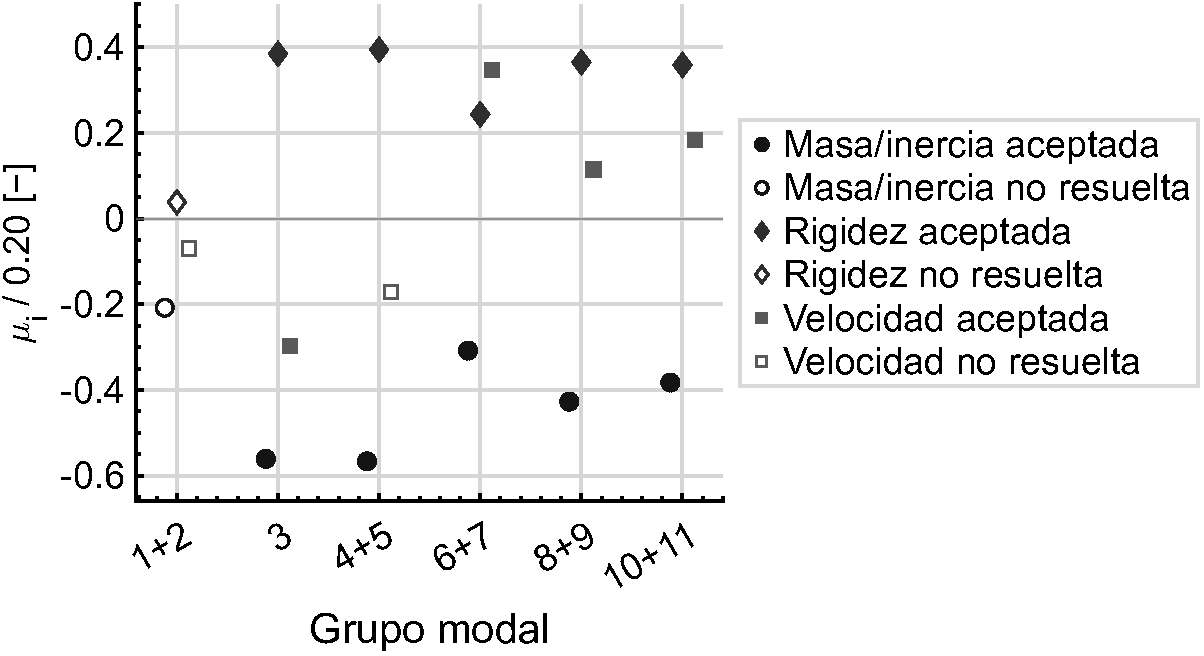
\includegraphics[width=.98\linewidth,height=.40\textheight,keepaspectratio]{figures/actualizacion_20261014/influencia_firmada_grupos.pdf}
\caption{Estimadores originales de Morris, con las etiquetas reales de los grupos. Se representa $\mu_i/0.20$; círculos para masa/inercia, diamantes para rigidez y cuadrados para velocidad. Los símbolos llenos indican influencia aceptada y los vacíos, no resuelta. El grupo 12 permanece excluido. La figura nueva conserva los datos del Morris y utiliza el estilo monocromático autorizado.}\label{fig:sentidos}
\end{figure}


La masa/inercia tiene signo negativo en todos los grupos aceptados y la rigidez, positivo. La velocidad tiene mayor magnitud relativa en 6+7, mientras que reduce la frecuencia de 3. El giro, por tanto, no produce un aumento universal de todas las frecuencias. La comparación de magnitudes es entre factores con el mismo ancho relativo y dentro de cada respuesta.

Para 10+11, la frecuencia nominal es $f_{d,0}=1.22543$ Hz y
\begin{equation}
\overline c_\rho=-0.38266,\qquad
\overline c_K=0.35860,\qquad
\overline c_\Omega=0.18389.
\end{equation}
Como orientación de magnitud, al aplicar $\Delta f_d\simeq f_{d,0}\overline c_i\Delta\xi_i$ a un aumento de 1\pct\ del factor se obtiene:
\begin{center}\small
\begin{tabular}{lrr}
\toprule Factor que aumenta & Cambio relativo orientativo & Cambio orientativo [Hz] \\ \midrule
Masa/inercia & -0.383\,\pct & -0.00469 \\
Rigidez & +0.359\,\pct & +0.00439 \\
Velocidad & +0.184\,\pct & +0.00225 \\

\bottomrule
\end{tabular}
\end{center}
Estos valores son ejemplos calculados a partir de secantes medias; \emph{no son nuevos casos a 1\pct\ ni predicciones locales certificadas}. Los signos y magnitudes son coherentes con las derivadas aceptadas de la primera etapa en el mismo grupo.

\subsection{Intervalos observados de frecuencia}
\begin{center}\small
\begin{tabular}{lrrr}
\toprule Respuesta & Nominal [Hz] & Mínimo observado [Hz] & Máximo observado [Hz] \\ \midrule
1+2 & 0.158 & 0.152 & 0.162 \\
3 & 0.231 & 0.205 & 0.263 \\
4+5 & 0.409 & 0.365 & 0.457 \\
6+7 & 0.587 & 0.536 & 0.641 \\
8+9 & 0.844 & 0.771 & 0.923 \\
10+11 & 1.225 & 1.116 & 1.342 \\

\bottomrule
\end{tabular}
\end{center}
Los extremos reúnen cambios simultáneos de los tres factores en los vértices calculados. No son intervalos de confianza ni extremos demostrados de todo el dominio continuo. En 10+11 se observaron 1.116--1.342 Hz. El rango observado en 1+2 existe, aunque sus influencias individuales no pasaron el filtro de ruido: observar variación y atribuirla con resolución suficiente son afirmaciones distintas.

\section{Qué mecanismos físicos respaldan las tendencias}
\subsection{Masa y rigidez: intuición y comprobación}
Como analogía, un oscilador escalar de masa $m$ y rigidez $k$ tiene $f=(2\pi)^{-1}\sqrt{k/m}$, de donde
\begin{equation}
\frac{\Delta f}{f}\simeq\frac{1}{2}\frac{\Delta k}{k}-\frac{1}{2}\frac{\Delta m}{m}.
\end{equation}
La relación explica por qué aumentar masa suele reducir frecuencia y aumentar rigidez suele elevarla. Es una analogía para interpretar signos; no sustituye el aerogenerador multicuerpo en rotación ni establece coeficientes exactos de $\pm0.5$ para sus factores.

En el modelo, $\xi_\rho$ cambia inercia traslacional y rotacional de palas, peso y contribuciones asociadas al giro; también cambia el equilibrio. $\xi_K$ modifica conjuntamente las rigideces axial, de cortante, torsional y de flexión. Los coeficientes observados incluyen acoplamiento con torre, góndola, cubo y conexiones, cuya masa y rigidez no se escalan en esta campaña. Por eso el efecto no se reduce a reemplazar toda la masa o toda la rigidez del sistema.

\begin{figure}[htbp]
\centering
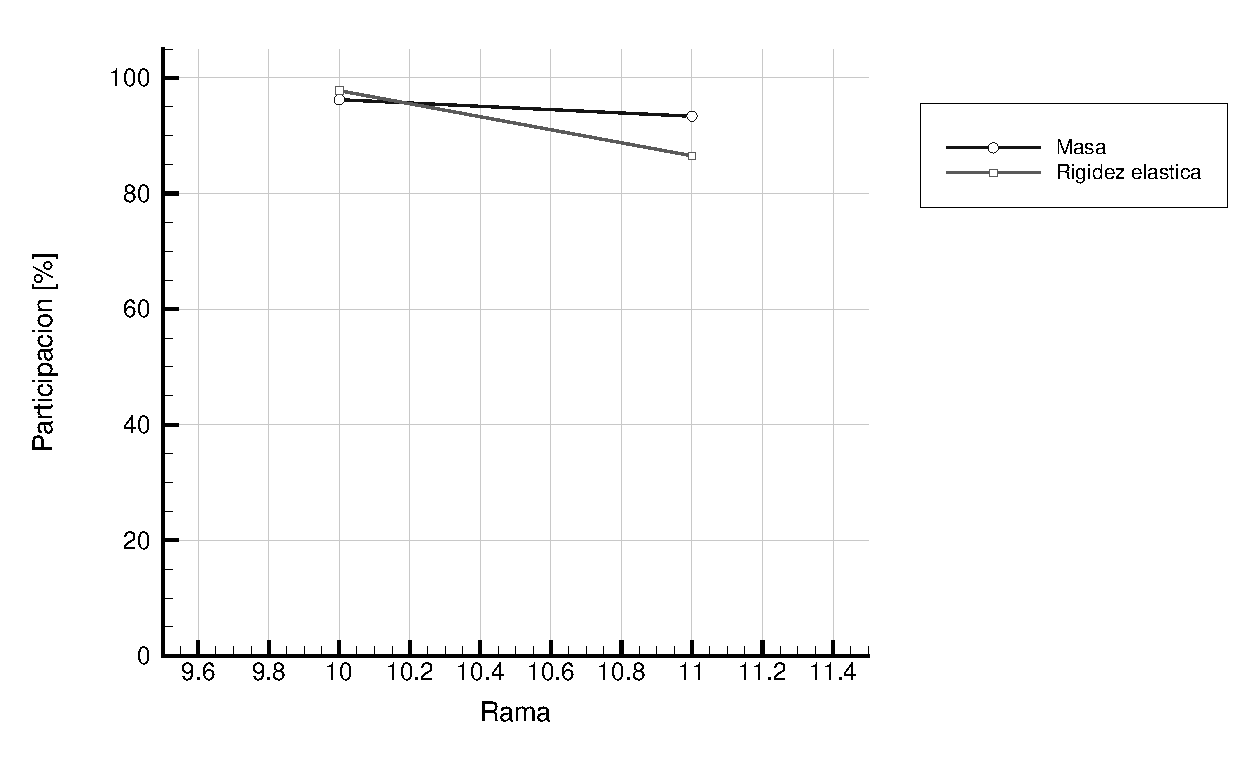
\includegraphics[width=.96\linewidth,height=.40\textheight,keepaspectratio]{figures/tecplot/morris_participaciones.pdf}
\caption{Comprobación mecánica independiente en la referencia de la primera etapa. Las palas aportan aproximadamente 96.2 y 93.4\pct\ de la forma cuadrática de masa, y 97.8 y 86.5\pct\ de la forma cuadrática elástica de las ramas 10 y 11. Se utilizan masa y rigidez elástica de referencia; no se representa toda la energía del sistema en rotación.}
\label{fig:participaciones}
\end{figure}


Para interpretar las participaciones de la figura~\ref{fig:participaciones}, sea $\boldsymbol\phi$ una forma nominal y $\mathsf M_c$ la contribución de masa del componente $c$. Su participación de referencia se obtiene de $\boldsymbol\phi^{\mathsf H}\mathsf M_c\boldsymbol\phi$ dividida por la suma de las contribuciones; $\mathsf H$ indica transposición conjugada. Se procede de forma análoga con la rigidez elástica de referencia. La presencia predominante de palas en 10 y 11 respalda la sensibilidad a sus propiedades. Estas participaciones no separan cuantitativamente todos los mecanismos de la tangente rotacional.

\subsection{Giro: competencia de contribuciones}
El incremento de velocidad modifica efectos giroscópicos proporcionales a $\Omega$, contribuciones inerciales y de transporte, términos proporcionales a $\Omega^2$, el equilibrio y las derivadas de las restricciones y de la transformación de coordenadas. La matriz de velocidad y la tangente intervienen simultáneamente en el problema cuadrático; no basta imaginar una rigidez adicional positiva.

El signo negativo observado en 3 y positivo en 6+7, 8+9 y 10+11 es evidencia de que la respuesta al giro depende del grupo. La hipótesis mecánica compatible con la formulación es una competencia de contribuciones cuya proyección modal cambia de una rama a otra. El cribado no identifica cuánto aporta individualmente cada término; esa separación requeriría un diagnóstico adicional del modelo existente.

\subsection{Compensación parcial entre masa y rigidez}
A velocidad fija, la orientación media del grupo 10+11 sugiere
\begin{equation}
\frac{\Delta f_d}{f_{d,0}}\simeq-0.38266\Delta\xi_\rho+0.35860\Delta\xi_K.
\end{equation}
Una cancelación aproximada de estas secantes daría $\Delta\xi_K\simeq1.067\Delta\xi_\rho$. Esta proporción es una \emph{hipótesis de compensación para comprobar}, no una ley válida para todos los puntos. Diferentes propiedades podrían producir frecuencias similares: ajustar solo una frecuencia puede dejar ambigüedad entre masa y rigidez.

\begin{figure}[htbp]
\centering
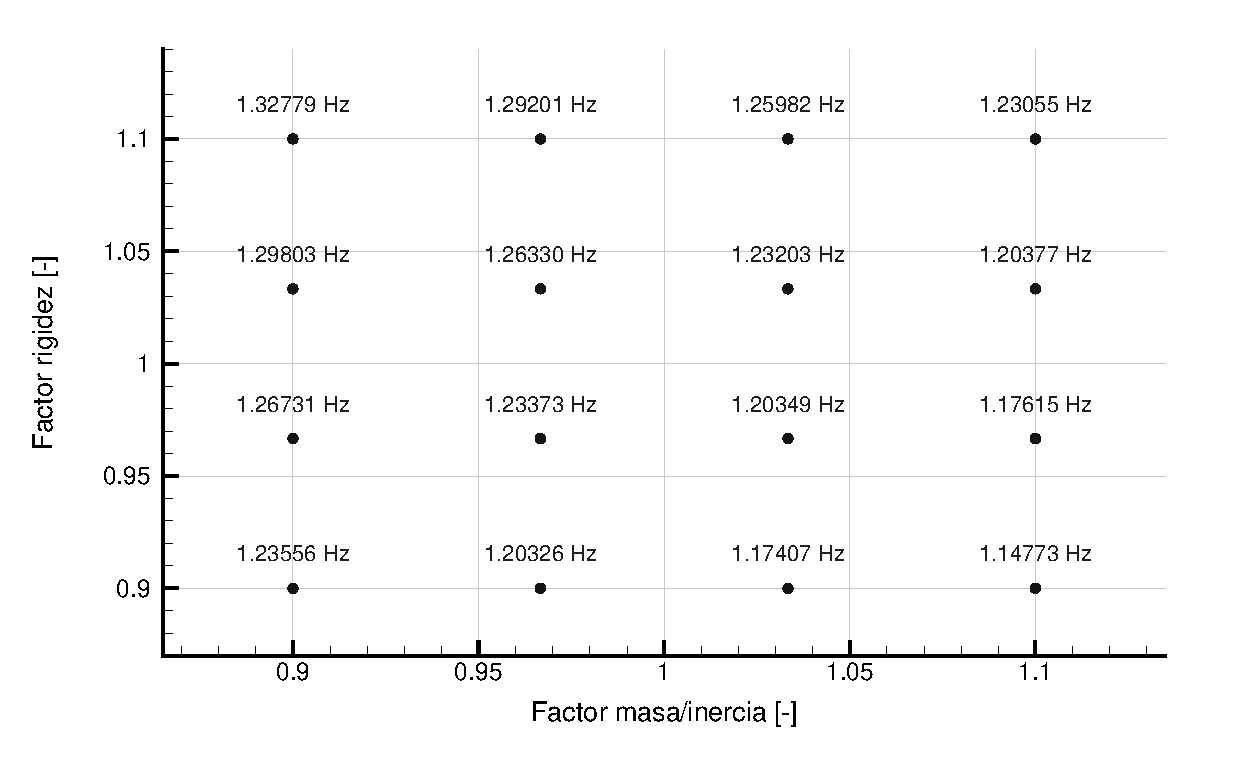
\includegraphics[width=.96\linewidth,height=.40\textheight,keepaspectratio]{figures/tecplot/morris_dominio.pdf}
\caption{Dieciséis combinaciones evaluadas a velocidad fija de 12.4 rpm. Cada punto y su etiqueta corresponden a una frecuencia media del grupo 10+11 almacenada. No se interpolan frecuencias entre puntos. Aumentar masa/inercia y aumentar rigidez producen efectos opuestos; la compensación diagonal es parcial.}\label{fig:dominio}
\end{figure}


La diagonal de la figura~\ref{fig:dominio} muestra frecuencias próximas al aumentar conjuntamente masa y rigidez. Por ejemplo, las esquinas de factores iguales $(0.90,0.90)$ y $(1.10,1.10)$ dan aproximadamente 1.236 y 1.231 Hz a 12.4 rpm. Los valores son cercanos, pero distintos; la compensación no es exacta. Sería útil contrastar más de una frecuencia, formas modales u otros indicadores al identificar propiedades.

\section{Por qué se aceptan unos resultados y otros no}
Se evalúan tres preguntas numéricas: ¿se sigue la misma respuesta modal?, ¿el efecto supera el ruido?, ¿el estimador se estabiliza al aumentar trayectorias? El éxito del solver no garantiza por sí solo las tres condiciones. En esta campaña, las formas y grupos cerrados se conservaron; el grupo abierto asociado a 12 se rechazó.

\subsection{Ruido y señal}
Sea $\eta$ la máxima diferencia de una respuesta observada entre controles: repetición nominal, tolerancia QEP más estricta y solución directa frente a continuación, en el nominal y dos esquinas. Se asigna la envolvente empírica por efecto
\begin{equation}
b_i^{(j)}=\frac{2\eta}{|\Delta x_i^{(j)}|s_y},\qquad
\overline b_i=\frac{1}{r}\sum_j b_i^{(j)}.
\end{equation}
La media absoluta debe satisfacer $\mu_i^*\geq10\overline b_i$. La envolvente no es una cota rigurosa de error en todo el dominio. La comparación con continuación es relevante porque diferencias pequeñas del equilibrio y la tangente pueden afectar indicadores aunque el residuo de equilibrio sea reducido.

\begin{figure}[htbp]
\centering
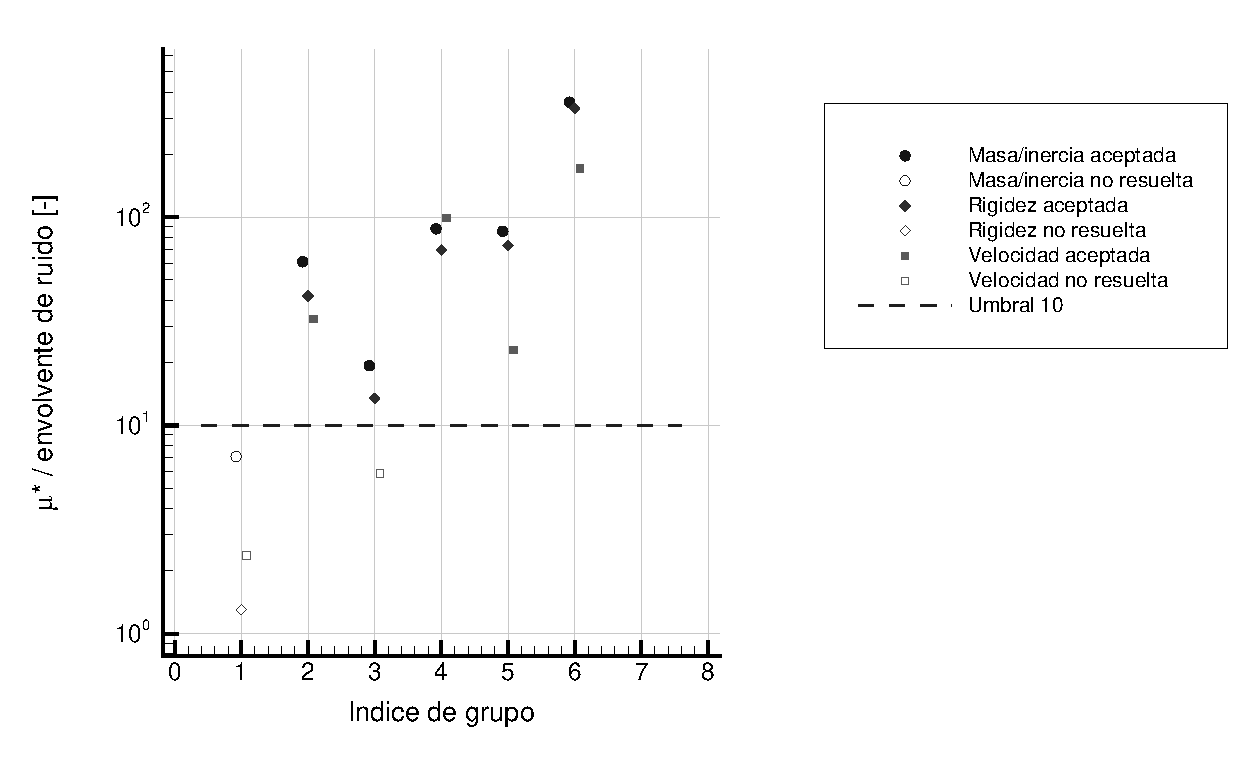
\includegraphics[width=.96\linewidth,height=.40\textheight,keepaspectratio]{figures/tecplot/morris_ruido.pdf}
\caption{Influencia frente a la envolvente empírica de ruido, en escala logarítmica. Se conserva el orden de grupos de la figura de secantes; la línea horizontal indica el umbral de aceptación 10. Los marcadores vacíos permanecen no resueltos. La estabilización de una media no basta para aceptarla.}\label{fig:ruido}
\end{figure}


Por ejemplo, para masa/inercia en 1+2 el cociente señal/ruido es 7.09 y, para velocidad en 4+5, 5.88: ambos quedan bajo el umbral 10. No se publican como influencias aceptadas, aunque sus estimadores cambian menos de 1\pct\ entre veinte y cuarenta trayectorias. Esto evita confundir una estimación repetible con una estimación suficientemente resuelta.

\subsection{Estabilización con el número de trayectorias}
\begin{figure}[htbp]
\centering
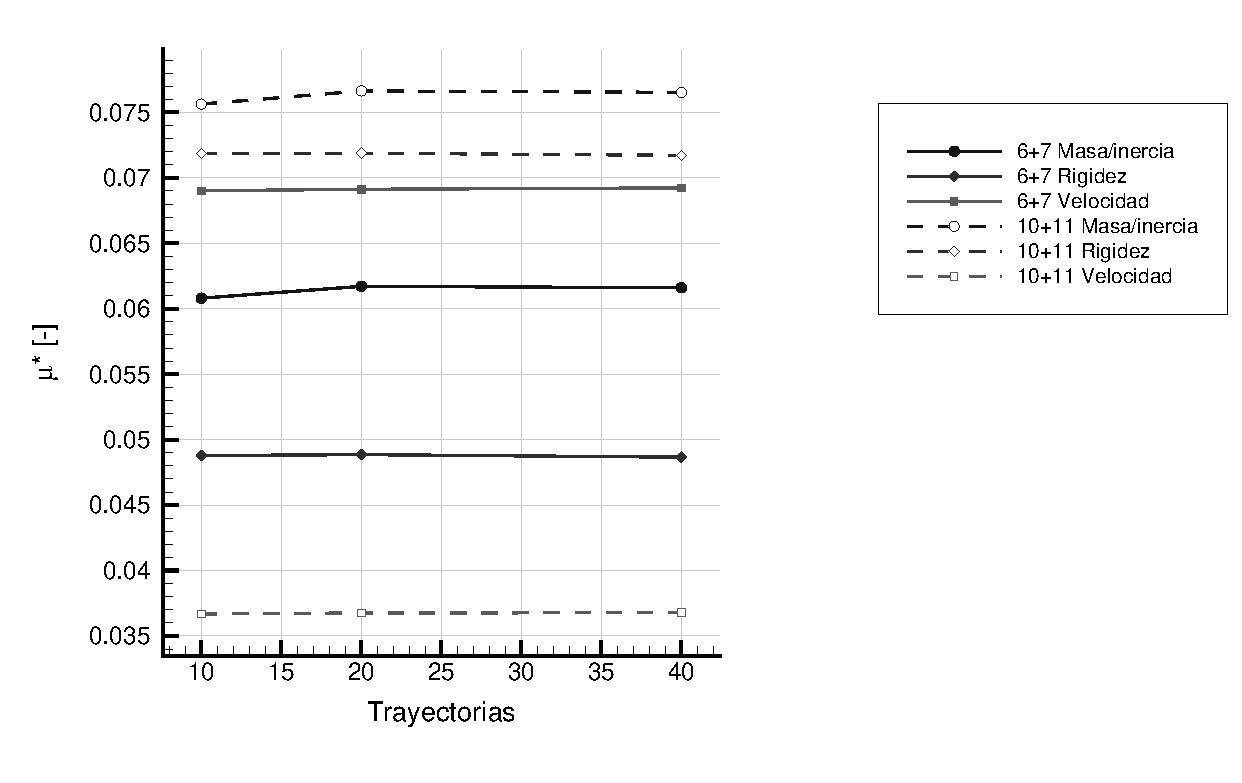
\includegraphics[width=.96\linewidth,height=.40\textheight,keepaspectratio]{figures/tecplot/morris_convergencia.pdf}
\caption{Estabilización de estimadores de los grupos 6+7 y 10+11 con prefijos de 10, 20 y 40 trayectorias del mismo diseño. Los símbolos distinguen factores y la leyenda identifica cada grupo. Las líneas unen prefijos calculados y no prueban convergencia asintótica.}\label{fig:convergencia}
\end{figure}


El máximo cambio relativo de $\mu_i^*$ entre veinte y cuarenta, entre los catorce indicadores aceptados, fue 0.80\,\pct. El umbral fijado era 10\pct. El orden de influencia se conserva en los grupos mostrados. Este resultado apoya la suficiencia del cribado para estas respuestas; no demuestra convergencia espacial de las sensibilidades en rotación ni elimina la dependencia de la malla numérica de Morris.

Los máximos residuos de equilibrio y del QEP en norma dual de masa fueron $9.94\times10^{-9}$ y $4.05\times10^{-9}$, respectivamente. Esta norma reúne fuerzas y momentos con una escala dimensional compatible. Las 170 evaluaciones convergieron y pasaron 17 pruebas del módulo. La regresión histórica de 155 pruebas se conserva como evidencia anterior; no se presenta como una nueva ejecución. Las 148 fuentes físicas MATLAB anteriores permanecieron intactas.

\section{Qué significa la dispersión aceptada}
\begin{figure}[htbp]
\centering
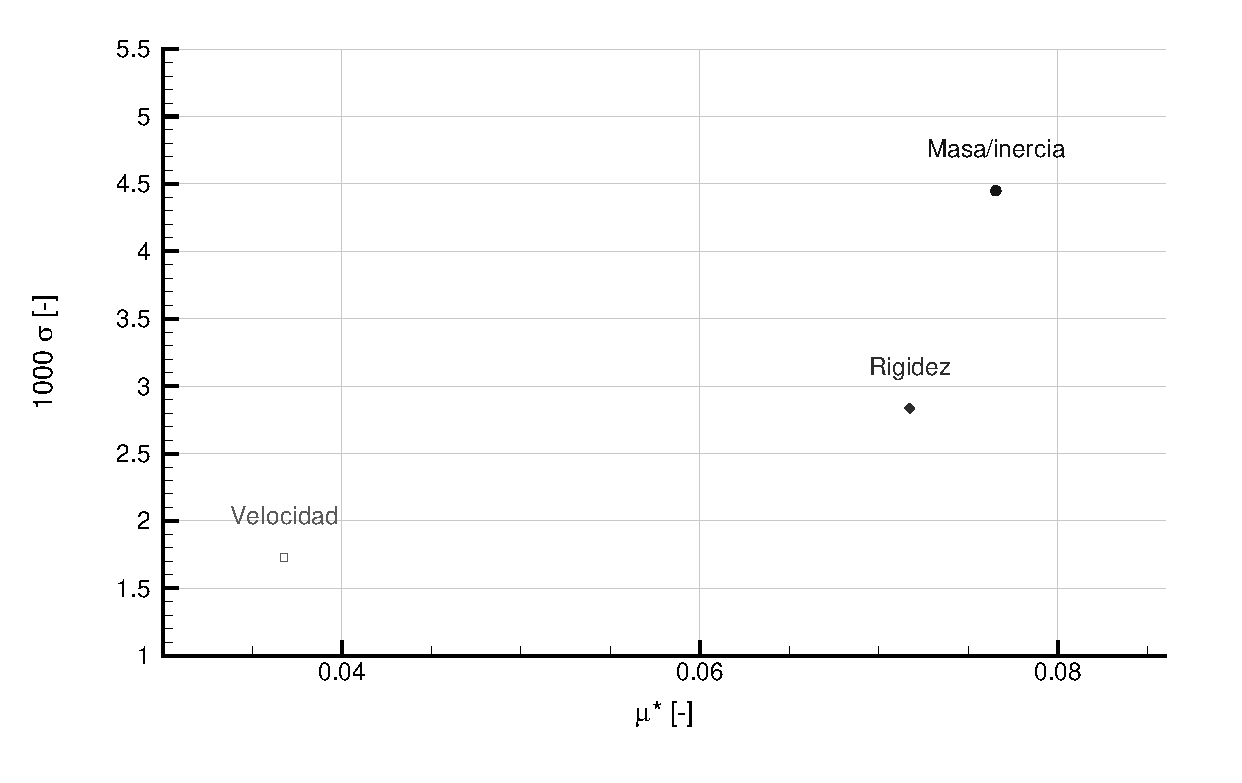
\includegraphics[width=.96\linewidth,height=.40\textheight,keepaspectratio]{figures/tecplot/morris_dispersion.pdf}
\caption{Influencia y dispersión de efectos elementales en el grupo 10+11. Los puntos llenos superan los controles de ruido y estabilización de $\sigma_i$; el punto vacío no. El eje vertical está multiplicado por $10^3$. Esta dispersión describe los efectos elementales, no una distribución física de frecuencias ni una probabilidad de fallo.}
\label{fig:dispersion}
\end{figure}


La dispersión indica que el efecto elemental cambia según el punto donde se evalúa. Puede reunir curvatura respecto del propio factor, dependencia de los otros factores e influencia numérica. Morris no separa estas causas. Para $\sigma_i$, la envolvente propagada es $b_{\sigma,i}=[\sum_j(b_i^{(j)})^2/(r-1)]^{1/2}$; se exige $\sigma_i\geq10b_{\sigma,i}$ y estabilización al 10\pct.

\begin{center}\small
\begin{tabular}{lrrrr}
\toprule Factor; grupo 10+11 & $\sigma_i$ & $\sigma_i/b_{\sigma,i}$ & Cambio 20--40 & Aceptado \\ \midrule
Masa/inercia & 0.00445 & 20.52 & 6.31\,\pct & Sí \\
Rigidez & 0.00283 & 13.07 & 8.22\,\pct & Sí \\
Velocidad & 0.00173 & 7.97 & 14.94\,\pct & No \\

\bottomrule
\end{tabular}
\end{center}
La dispersión de masa/inercia y rigidez supera el ruido y cambia aproximadamente 6.31\pct\ y 8.22\pct, respectivamente. La de velocidad tiene cociente 7.97 y no supera el filtro de ruido. No puede afirmarse que el giro sea exactamente lineal o independiente de los otros factores por ese rechazo. Tampoco puede afirmarse que las dos dispersiones aceptadas demuestren, por sí solas, una interacción específica.








% BEGIN COMPLEMENT 20261014
\clearpage
\section{Comprobación complementaria de la rejilla y de los efectos combinados}
\subsection{Cobertura, controles y conservación del modelo}
La rejilla de cuatro niveles y tres factores contiene $4^3=64$ combinaciones. Morris había visitado 58 combinaciones distintas. Se resolvieron las seis faltantes y tres controles: QEP más estricto y continuación en uno de esos puntos, y repetición nominal. Se conservaron los casos de Morris y sus estimadores. Las nueve evaluaciones nuevas tomaron 77.49 s de solve, bajo un límite operacional de 300 s. La campaña modal global reúne así 170 evaluaciones originales y nueve complementarias, con 64 puntos de rejilla distintos.

Se verificaron las 175 huellas de fuentes de la campaña original. Los grupos históricos se conservan y sus formas pasan las comprobaciones correspondientes. La rama 12 continúa abierta frente a ramas fuera del conjunto seguido y queda excluida. Los rangos físicos, propiedades vinculadas y formulación permanecen iguales. La continuación y el QEP estricto en un nuevo punto no aumentaron la envolvente de frecuencia de 10+11: $\eta=8.7456\times10^{-5}$ Hz. La diferencia máxima de sus controles nuevos fue $1.0613\times10^{-5}$ Hz.

Las medias de secantes de extremos conservan el orden de influencia de los cinco grupos principales. Sus pasos y ponderaciones difieren de Morris, de modo que no son estimadores idénticos ni derivadas infinitesimales. En 1+2, la media absoluta de secantes de masa de extremo tiene cociente señal/ruido 10.41, cercano al umbral 10; solo once de sus dieciséis comparaciones individuales superan ese umbral. Este resultado marginal no cambia retrospectivamente la ausencia de aceptación de su estimador Morris.

\subsection{Compensación parcial a las cuatro velocidades}
Se examina la diagonal $\xi_\rho=\xi_K$ a 10.8, 11.6, 12.4 y 13.2 rpm. El cambio entre factores iguales 0.90 y 1.10 es de aproximadamente 0.00495--0.00519 Hz, equivalente a 0.404--0.423\pct\ de $f_{d,0}$ de 10+11. Cada curva de la figura usa como origen su propio punto diagonal 0.90. La cercanía de frecuencias apoya una compensación parcial, pero no una identidad válida para toda la respuesta. La identificación de propiedades necesita otras frecuencias, formas u observaciones.
\begin{figure}[htbp]\centering
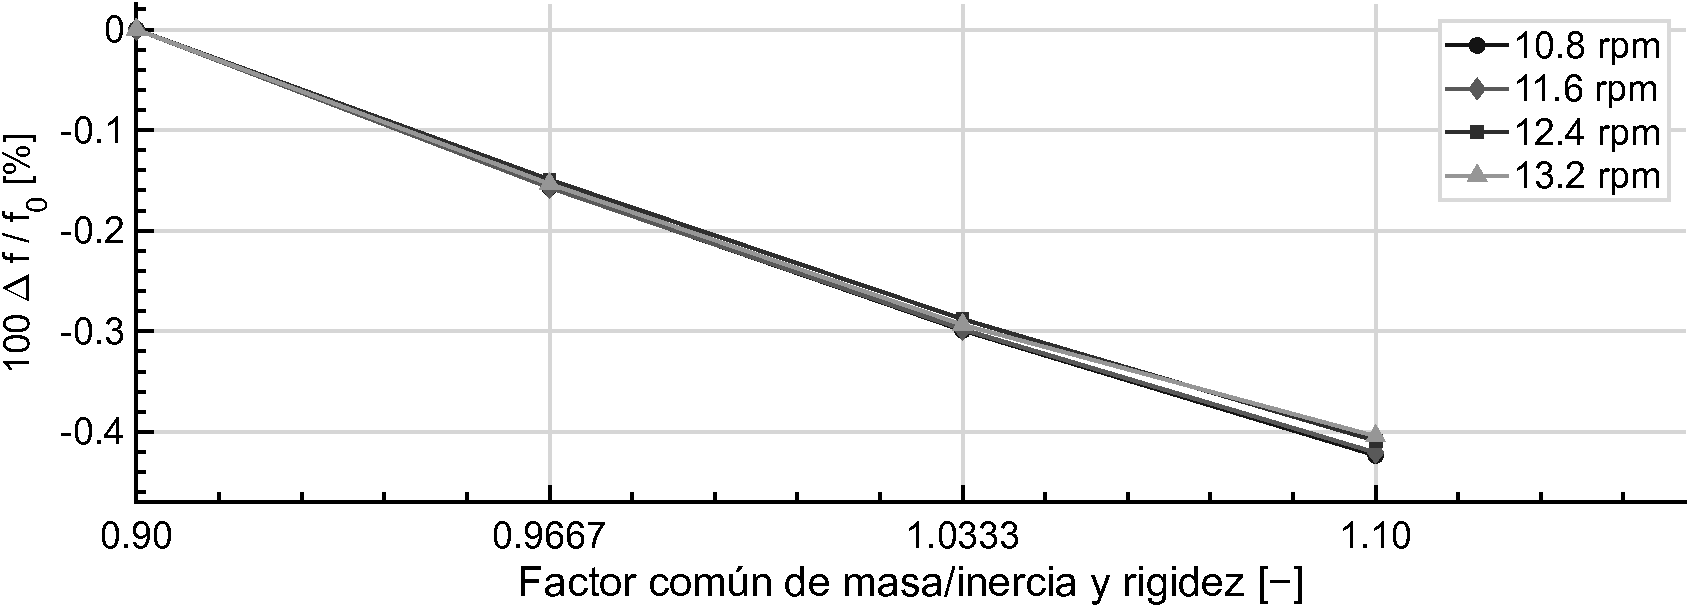
\includegraphics[width=.92\linewidth,height=.37\textheight,keepaspectratio]{figures/actualizacion_20261014/compensacion_rejilla.pdf}
\caption{Cambios de frecuencia de 10+11 a lo largo de la diagonal masa--rigidez, medidos respecto del punto 0.90 de cada velocidad y normalizados por la frecuencia nominal fija. Se muestran únicamente valores calculados de la rejilla; las líneas conectan esos valores.}\label{fig:compensacion-rejilla}
\end{figure}
\FloatBarrier

\subsection{Contraste rectangular para distinguir no aditividad}
Para dos factores $i,j$, con el tercero fijo, se calcula el contraste de sus extremos:
\begin{equation}
I_{ij}=f_{++}-f_{+-}-f_{-+}+f_{--}.
\end{equation}
Los signos indican factores 1.10 y 0.90. Si la respuesta fuera una suma de funciones separadas de los dos factores, el contraste sería cero, incluso si dichas funciones tuvieran curvatura individual. Un contraste resuelto evidencia no aditividad de esta respuesta en esos puntos. No atribuye un mecanismo concreto a un término del operador ni cuantifica un porcentaje de varianza.

La envolvente propagada es $b_I=4\eta$, por los cuatro términos del contraste. Se exige $|I_{ij}|\geq10b_I$, además de seguimiento válido. La cota continúa siendo empírica. Para 10+11 se obtiene:
\begin{center}\small
\begin{tabular}{lrrl}\toprule
Par & $|I_{ij}|$ [Hz] & $|I_{ij}|/b_I$ & Interpretación \\ \midrule
Masa--rigidez & 0.00926--0.00940 & 26.47--26.87 & Resuelto \\
Masa--velocidad & 0.00356--0.00362 & 10.17--10.34 & Marginal sobre el umbral \\
Rigidez--velocidad & 0.00331--0.00342 & 9.47--9.77 & No resuelto \\
\bottomrule\end{tabular}
\end{center}
Masa--rigidez presenta contraste negativo en las cuatro velocidades. El incremento de rigidez tiene menor efecto de frecuencia al aumentar masa, de forma compatible con la dependencia conjunta de rigidez e inercia. La afirmación se limita al contraste observado, no a una separación causal de todos los operadores. Masa--velocidad supera por poco el umbral y requiere cautela. Rigidez--velocidad permanece sin resolución suficiente; no se infiere ausencia de interacción.
\begin{figure}[htbp]\centering
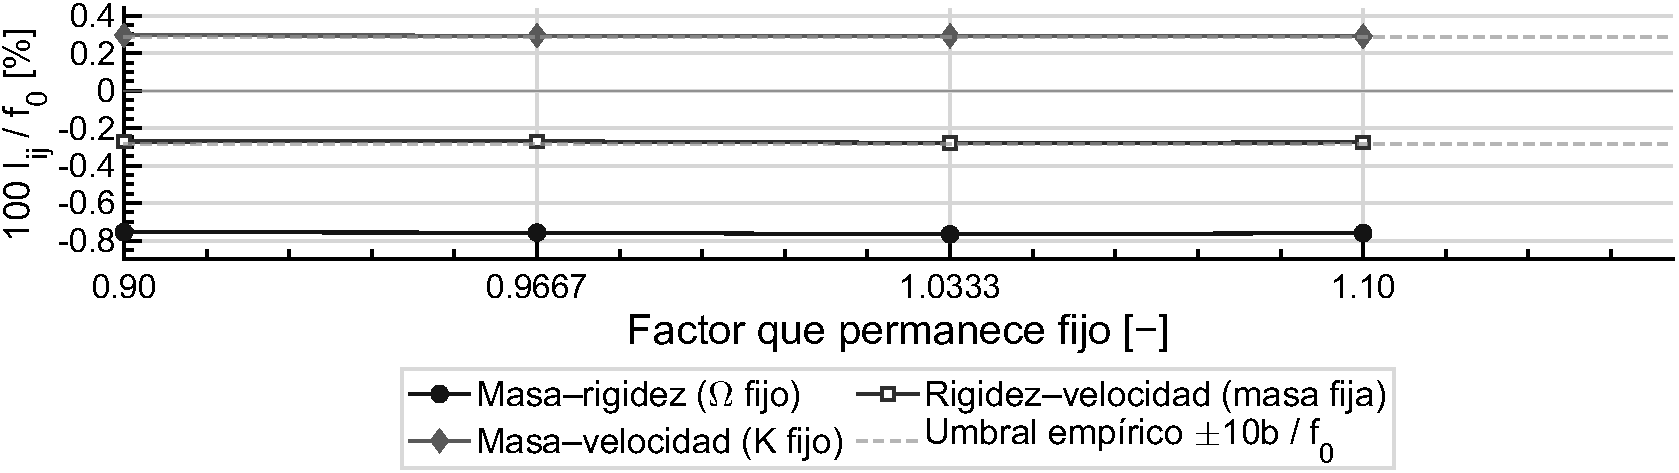
\includegraphics[width=.98\linewidth,height=.38\textheight,keepaspectratio]{figures/actualizacion_20261014/contrastes_interaccion.pdf}
\caption{Contrastes de extremos en 10+11, normalizados por $f_{d,0}$. Cada curva deja fijo un factor diferente, identificado en la leyenda. Los símbolos llenos superan el umbral empírico y los vacíos no. Las líneas discontinuas muestran $\pm10b_I/f_{d,0}$ en porcentaje.}\label{fig:contrastes-interaccion}
\end{figure}
\FloatBarrier

\subsection{Curvatura individual y límites de esta comprobación}
En pasos igualmente espaciados se calcula $C_i=f_{i+1}-2f_i+f_{i-1}$. En 10+11, seis de los 32 contrastes de masa/inercia superan diez veces la envolvente $4\eta$. Ninguno de los 32 contrastes de rigidez o de velocidad supera ese filtro. Por tanto, la evidencia adicional resuelve curvatura de masa en ciertos puntos y no aditividad masa--rigidez; las restantes ausencias de resolución no prueban linealidad.

El contraste masa--velocidad es un indicador diferente de $\sigma_\Omega$ de Morris, cuya aceptación original sigue siendo negativa. La rejilla completa verifica todos sus 64 puntos discretos, sin certificar extrema o monotonicidad del dominio continuo, convergencia espacial en operación ni incertidumbre probabilística. Sus tablas guardan también todos los indicadores que no superan el filtro.

La licencia de Tecplot vencida impidió exportaciones nuevas. El autor autorizó el 14 de octubre utilizar las figuras ya generadas y producir las restantes con el mismo formato y estilo. Se exportaron tres figuras nuevas y cuatro adaptaciones de legibilidad para la presentación con MATLAB R2026a, en escala de grises, fondo blanco y PDF vectorial. Su catálogo registra motor, datos y procedencia. Las figuras anteriores conservan su procedencia Tecplot.
% END COMPLEMENT 20261014

% BEGIN REAL INPUTS 20261020
\FloatBarrier
\section{Comparación con entradas medidas: sismo y viento}
Esta etapa extiende el estudio a historias temporales medidas. El autor autorizó utilizar registros de fuentes independientes y representar el viento mediante un empuje axial prescrito cuyo valor medio permanece como parámetro. Se cierra así una comparación estructural determinista y reproducible; el empuje medio real de la turbina y su respuesta aeroelástica acoplada siguen sin identificarse. Se conservan los resultados Morris anteriores y sus condiciones de aceptación.

\subsection{Literatura, datos disponibles y nivel de comparación}
Wang y colaboradores~\cite{wang2026inputs} publican ambas entradas de su análisis: registros sísmicos PEER y viento sintético de Davenport. Se descargaron y verificaron los archivos de su repositorio~\cite{diao2026data}, cuya versión comprobada contiene proyectos Origin OPJU. No se extrajeron de esos proyectos series numéricas ni se reprodujo su turbina híbrida de 160 m. Esta referencia sustenta la organización de casos, pero no acredita dos entradas de campo medidas.

Meng y colaboradores~\cite{meng2020} estudian experimentalmente viento y excitación de mesa sísmica, y muestran la importancia del amortiguamiento aerodinámico para combinar acciones. Turello y colaboradores~\cite{turello2023inputs} estudian un sismo derivado de Loma Prieta, ajustado a un espectro de diseño, y cargas calculadas con un modelo aeroelástico. Ninguno de esos tratamientos se sustituye aquí por un amortiguamiento aerodinámico supuesto.

Para las entradas medidas se seleccionaron el conjunto NM92 de DTU~\cite{dtu2021inputs} y acelerogramas procesados distribuidos en el repositorio oficial de OpenSees~\cite{openseesinputs}. El registro eólico y los sismos no ocurrieron juntos. Tampoco se comparan mediciones de respuesta de una misma turbina con predicciones: el nivel de comparación es el de \emph{entradas transferidas al modelo existente}, con sus hipótesis declaradas.

\subsection{Qué se midió y cómo se preparó}
El viento corresponde al primer archivo disponible en orden lexicográfico, fechado el 19 de noviembre de 2005 a las 00:00 según su cabecera; la zona horaria no está indicada. Se emplea el canal sónico longitudinal \texttt{s70u}, a 70 m de altura, con 15\,000 muestras a 25 Hz. La duración de adquisición es 600 s y la separación entre primera y última muestra es 599.96 s. Se verificaron las estadísticas contra la cabecera: media 6.1341 m/s, desviación poblacional 0.2604 m/s e intensidad longitudinal $I_u=\sigma_u/\overline U=4.246\pct$. Es un registro seleccionado de viento relativamente uniforme; no representa por sí solo condiciones extremas.

La turbina medida es una NEG-Micon NM92 de 2.75 MW, cuyo registro indica 14.65 rpm. El escenario estructural conserva sus 12 rpm prescritas. La historia a 70 m se utiliza como sustituto temporal de un viento uniforme autorizado, sin extrapolación de altura ni afirmación de que se haya medido en el buje de este modelo. Los canales sónicos de 47 y 24 m aparecen duplicados en el archivo y no se usan para inferir un perfil espacial. Los momentos de palas, eje y torre publicados por DTU son respuestas internas medidas, no fuerzas nodales externas directamente transferibles.

Los acelerogramas conservan sus muestras, amplitudes y procesamiento de origen. El importador comprueba número de puntos, paso y unidades; convierte $g$ a m/s$^2$ mediante $g_0=9.80665$ m/s$^2$. No aplica escalamiento adicional ni corrección de línea base. Se interpolan linealmente las aceleraciones para integrar. Se emplea una componente horizontal por vez en X o Y; no se inventan componentes verticales ni se atribuye esa orientación a un emplazamiento real. No se interpretan desplazamientos absolutos del terreno obtenidos por doble integración como magnitudes validadas.

\begin{figure}[htbp]\centering
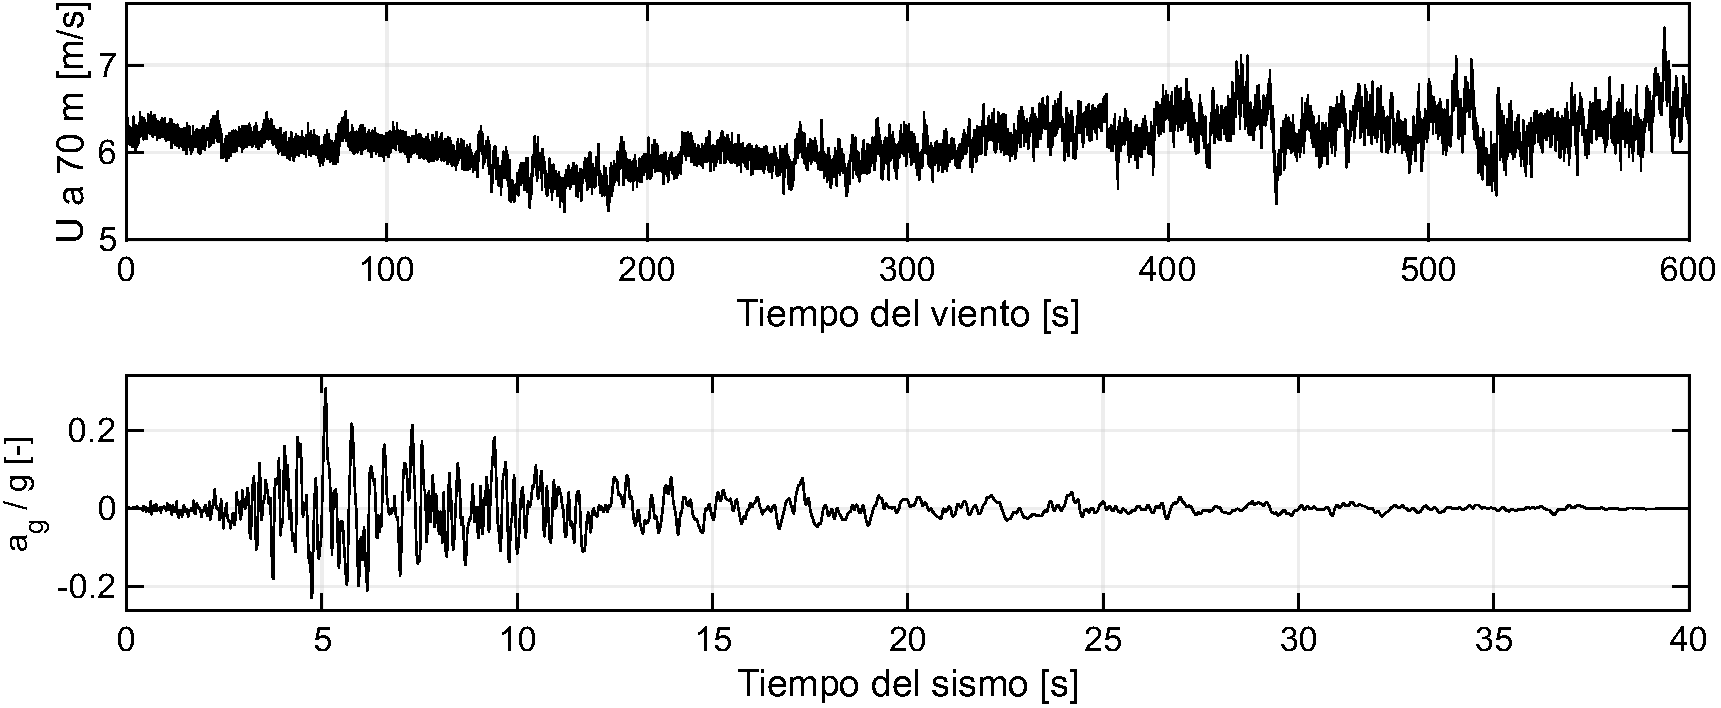
\includegraphics[width=.96\linewidth]{../entradas_reales_20261020/figures/entradas_medidas.pdf}
\caption{Historias medidas usadas como fuentes independientes. Los ejes temporales pertenecen a cada adquisición; sus amplitudes tienen unidades diferentes y no comparan directamente severidad de las acciones.}\label{fig:entradas-reales}
\end{figure}
\FloatBarrier

\subsection{De velocidad de viento a empuje parametrizado}
Sea $\overline F$ el empuje medio muestral, $U_n$ las muestras originales del viento y $N=15000$. Se prescribe
\begin{equation}
g_w(t_n)=\frac{U_n^2}{N^{-1}\sum_{j=1}^N U_j^2},\qquad
\boldsymbol f_{w,\mathrm{full}}(t)=\overline F\,\boldsymbol b_{\mathrm{full}}\,g_w(t),
\end{equation}
donde $\boldsymbol b_{\mathrm{full}}$ aplica una fuerza axial unitaria en el maestro del buje 130 según el eje 129--130. Se interpola $g_w$ a partir de sus muestras originales; no se vuelve a elevar al cuadrado una velocidad ya interpolada. No se fija $C_T$, densidad del aire ni área efectiva para deducir un empuje real. La respuesta se calcula por 1 kN de $\overline F$.

Esta aproximación corresponde a un empuje impuesto proporcional a $U^2$, con forma espacial concentrada en el buje. No incorpora inducción, cargas distribuidas en las palas, arrastre de la torre, control de paso o realimentación del movimiento sobre el flujo. Tampoco es una implementación de BEM. Esas capacidades requieren información aerodinámica específica adicional.

Con los operadores congelados de cada caso mecánico, la ecuación integrada es
\begin{equation}
\mathsf M\ddot{\boldsymbol q}+\mathsf D\dot{\boldsymbol q}+\mathsf K\boldsymbol q
=-\mathsf P_g a_g(t-\tau)+\overline F\,\boldsymbol b\,g_w(t),
\qquad
\mathsf P_g=\mathsf T_c^T\mathsf M_{\mathrm{full}}\boldsymbol R_g,\quad
\boldsymbol b=\mathsf T_c^T\boldsymbol b_{\mathrm{full}}.
\end{equation}
Aquí $\boldsymbol R_g$ contiene la traslación absoluta de base y $\tau$ es el instante de llegada del sismo en el reloj del viento. La fuerza sísmica se reconstruye al cambiar la masa; no se mantiene artificialmente constante.

Para viento se adopta como condición inicial el equilibrio \emph{lineal} $\mathsf K\boldsymbol q_{w,0}=\overline F\boldsymbol b$, con velocidad perturbada nula; la aceleración inicial satisface la ecuación con el primer valor real de $g_w$. El equilibrio por gravedad y giro se recalcula para cada factor mecánico, pero los operadores no se actualizan por un empuje finito ni durante la historia. Por eso la proporcionalidad respecto de $\overline F$ describe este problema lineal congelado, no una familia completa de estados operativos aeroelásticos.

Las recuperaciones nodales conservan $\mathsf T_c$, $\dot{\mathsf T}_c$ y $\ddot{\mathsf T}_c$ de una misma instantánea. Se calculan desplazamientos relativos y aceleraciones absolutas, añadiendo a estas últimas la aceleración de base correspondiente. Mantener esos términos de transporte no hace evolucionar el azimut.

\subsection{Contenido frecuencial y comparación sísmica}
La figura~\ref{fig:espectros-reales} compara formas espectrales normalizadas a integral unitaria: aceleración del suelo y fluctuación de $g_w$. Se usa Welch con ventanas de 20 s, ventana de Hann y solape del 50\pct. La normalización permite comparar distribución de frecuencia, no iguala fuerzas, energía o peligrosidad. La estimación de viento dispone de más segmentos que la del registro de Arleta.
\begin{figure}[htbp]\centering
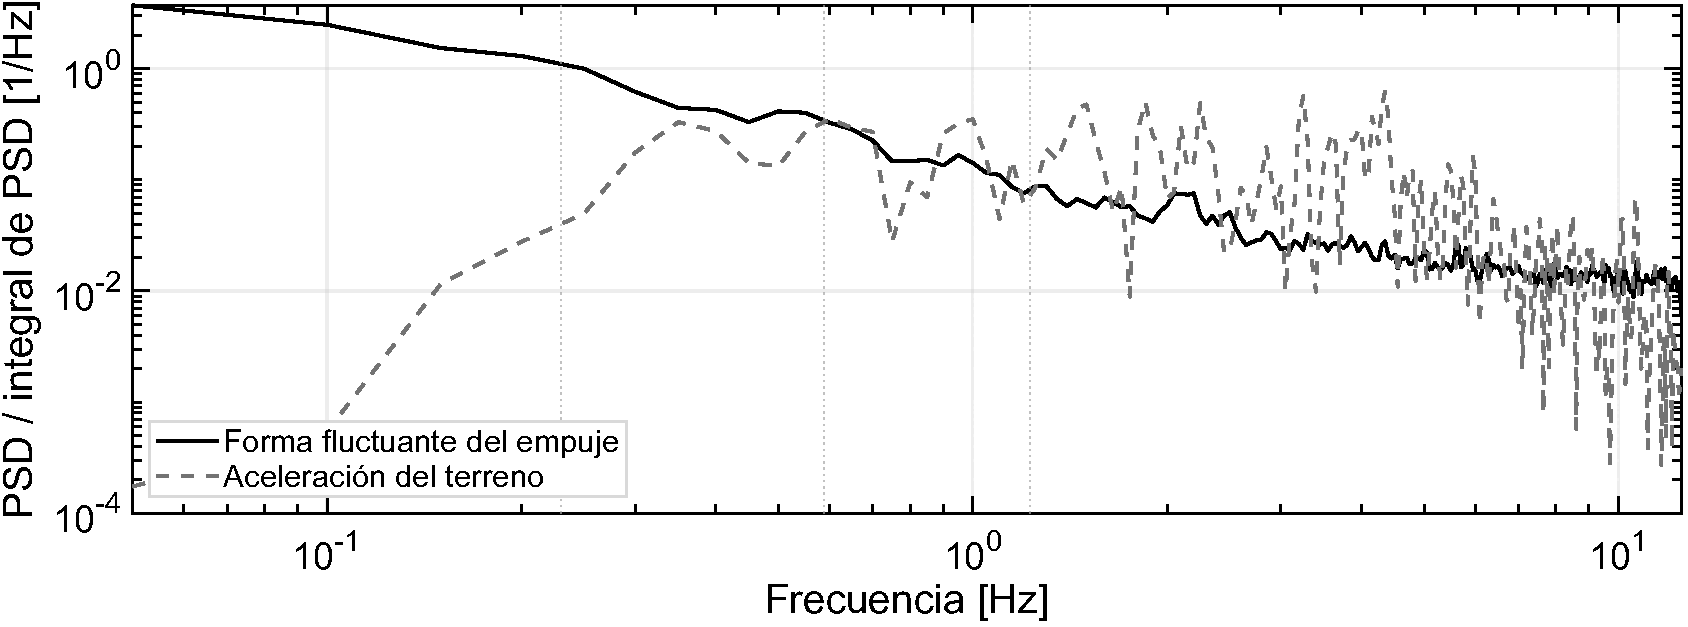
\includegraphics[width=.96\linewidth]{../entradas_reales_20261020/figures/contenido_frecuencial.pdf}
\caption{Distribución espectral normalizada de las entradas. Las líneas verticales indican frecuencias nominales de 3, 6+7 y 10+11; la proximidad espectral no sustituye las participaciones modales ni la proyección de cargas.}\label{fig:espectros-reales}
\end{figure}

La tabla compara los tres registros con amplitud original, aplicados en X. Corresponden a \emph{dos terremotos}, con dos estaciones distintas de Chi-Chi. Las duraciones completas son distintas: 39.98, 147.996 y 89.995 s. El cociente desplazamiento/PGA es una normalización diagnóstica del problema lineal, no una respuesta normalizada a un espectro de diseño común.
\begin{center}\small
\begin{tabular}{p{5.2cm}rrrr}
\toprule Registro & PGA [$g$] & $q_{H,\max}$ [m] & $a_{H,\max}^{\mathrm{abs}}$ [m/s$^2$] & $q_{H,\max}$/PGA [m/$g$]\\\midrule
Northridge, Arleta (1994) & 0.3081 & 0.2831 & 0.5792 & 0.919 \\
Chi-Chi, CHY023-W (1999) & 0.0467 & 0.1869 & 0.2283 & 4.004 \\
Chi-Chi, TCU052-N (1999) & 0.4190 & 1.9113 & 2.2327 & 4.561 \\
\bottomrule\end{tabular}\end{center}
No se puede atribuir la diferencia de respuesta únicamente a la PGA: cambian espectro, duración y estación. Estos casos tampoco cuantifican la amenaza de un sitio particular.
\begin{figure}[htbp]\centering
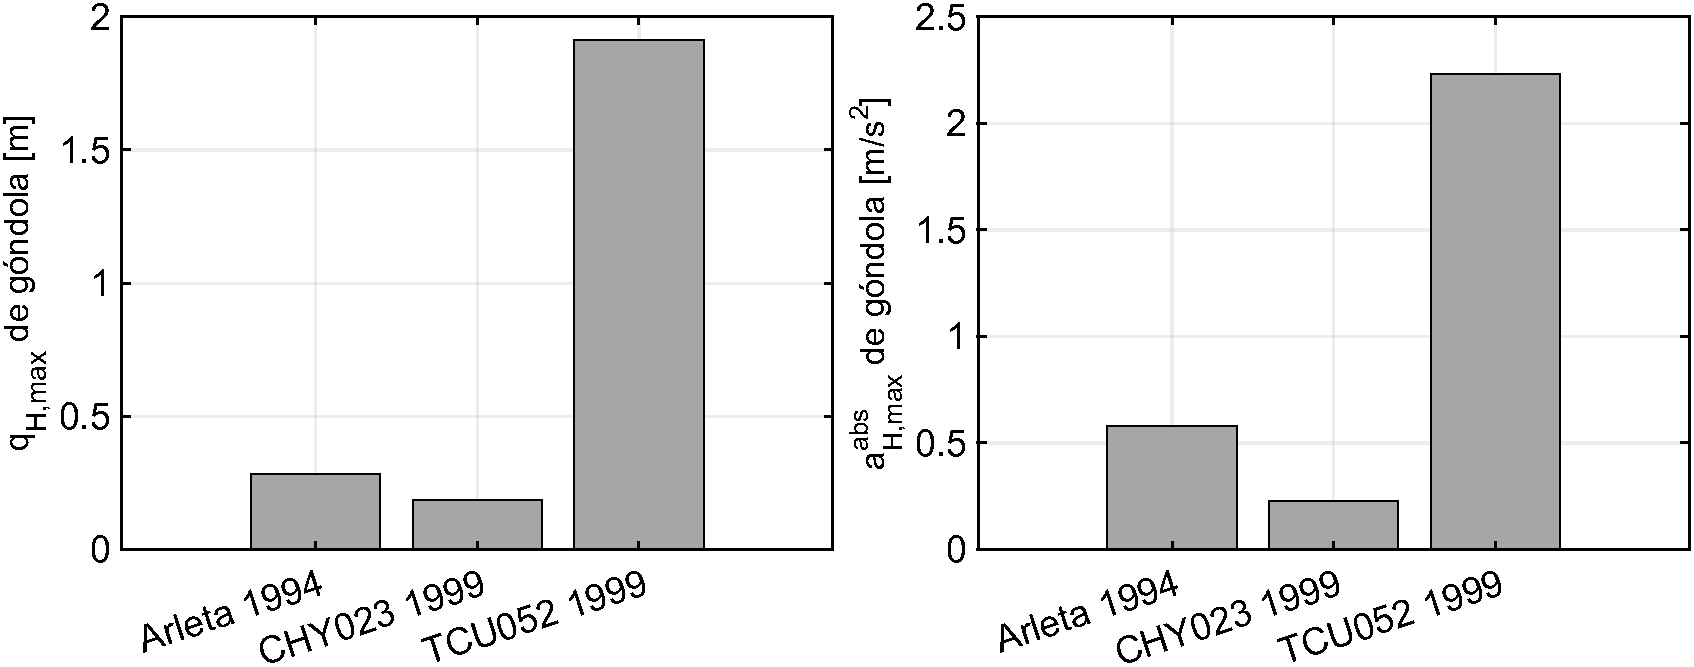
\includegraphics[width=.96\linewidth]{../entradas_reales_20261020/figures/respuesta_sismos_reales.pdf}
\caption{Máximos horizontales de góndola con cada registro completo aplicado en X, sin escalar. Se distinguen desplazamiento relativo y aceleración absoluta.}\label{fig:respuesta-sismos-reales}
\end{figure}
\begin{figure}[htbp]\centering
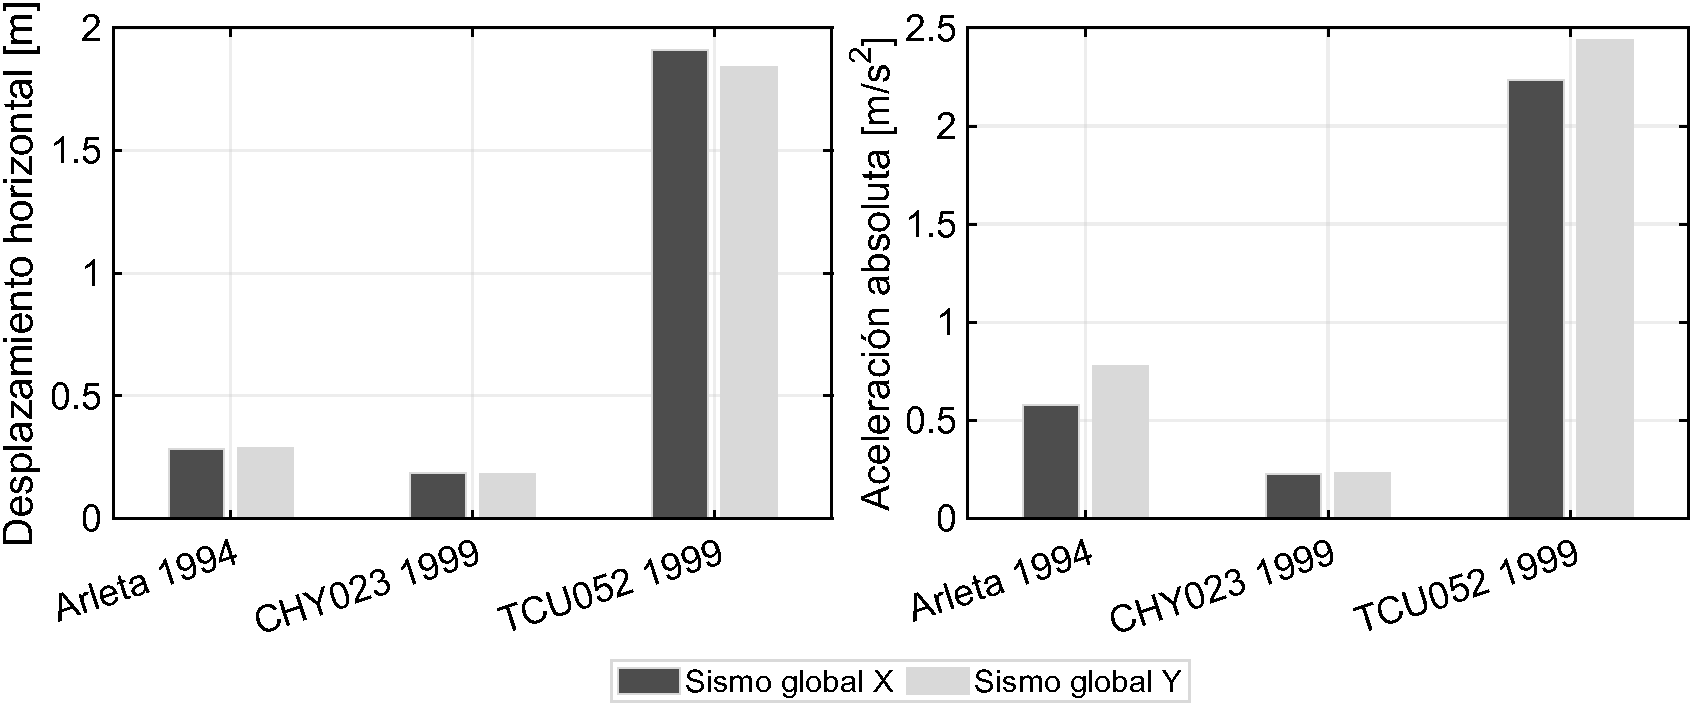
\includegraphics[width=.96\linewidth]{../entradas_reales_20261020/figures/efecto_direccion.pdf}
\caption{Efecto de aplicar la misma componente sísmica en X o Y. X corresponde al plano vertical que contiene el eje del rotor; Y es transversal. Esta es una comparación de orientación del escenario, no una simulación bidireccional observada.}\label{fig:direccion-reales}
\end{figure}
\FloatBarrier

\subsection{Qué resultados temporales son comparables}
Se define $q_H(t)=\sqrt{q_x^2+q_y^2}$ en la góndola 129, y análogamente $a_H^{\mathrm{abs}}$. Los máximos describen la mayor demanda durante la ventana. Como indicador complementario se usa
\begin{equation}
q_{H,\mathrm{RMS}}=\left[\frac1T\int_0^T(q_x^2+q_y^2)\,dt\right]^{1/2},
\end{equation}
y expresiones equivalentes para aceleración horizontal y momento flector de base. El RMS mide magnitud cuadrática media; en viento incluye la componente media del empuje y no es la desviación de la fluctuación alrededor de la media.

Las sensibilidades mecánicas comparan los primeros 39.98 s de Arleta y del viento, manteniendo para este último la normalización con las 15000 muestras del registro completo. Se estudiaron masa/inercia de palas, sus seis rigideces y velocidad prescrita. Se recalculó el estado heredado y el conjunto de operadores en cada caso.

El análisis inicial con $h=1\pct$ y $0.5\pct$ mostró dependencia importante del paso en numerosos máximos. Se añadieron $h=0.25\pct$ y $0.125\pct$; la tabla siguiente usa $0.25\pct$ y contrasta con $0.5\pct$, después de refinar la Hessiana interna. También se comparan pasos temporales de 0.005 y 0.0025 s. No se confunde un máximo bien convergido en tiempo con una derivada respecto del parámetro bien resuelta.

\subsubsection*{Verificación adicional de la Hessiana interna}
La rutina heredada aproxima primeras y segundas derivadas de una energía escalar con pasos internos de $2\times10^{-6}\max(L,1\ \mathrm{m})$ en traslación y $2\times10^{-6}$ rad en rotación. Se conservó el equilibrio convergido original y se sustituyó solamente la Hessiana interna almacenada en la tangente dinámica, usando pasos internos multiplicados por 20; se contrastó con un factor 40. La energía, las cargas y sus proyecciones no se modificaron. No se cambió ninguna de las 175 fuentes congeladas: esta opción numérica vive en el adaptador nuevo. Se ejecutaron 54 casos adicionales para aislar este efecto. Además de los controles de perturbación y Newmark, se exige variación de la pendiente inferior al 2\pct\ entre factores internos 20 y 40 y variación nominal inferior al 1\pct. La envolvente empírica de la pendiente se construye con las diferencias de cada extremo perturbado entre ambas Hessianas, no solo con repetición del nominal. En 22 de 90 indicadores las pendientes son estables con los pasos examinados. Se aceptan 1 de 90 indicadores al añadir la envolvente conservadora. Esta envolvente suma diferencias absolutas en los extremos sin cancelar el sesgo común entre discretizaciones; no es una estimación probabilística ni una cota demostrada. Por eso una pendiente estable respecto de los pasos puede permanecer sin aceptación completa. No se utiliza este conjunto para proclamar un orden global de parámetros. La tabla de máximos entre terremotos y la franja de llegadas conservan la configuración heredada, identificada en sus archivos; esta verificación adicional distingue la resolución de las derivadas sin sustituir retrospectivamente esas corridas ni el estudio Morris.

Se acepta cada sensibilidad local únicamente si el cambio relativo al duplicar $h$ y al duplicar $\Delta t$ es como máximo del 2\pct, los controles nominales a 0.0025 y 0.00125 s difieren como máximo del 1\pct\ en máximo y norma temporal, y la señal supera diez veces la envolvente empírica entre ambas Hessianas. Esa envolvente se estima en los extremos perturbados y no constituye una cota rigurosa del dominio. Se aceptan 1 de 90 indicadores locales: 1 de máximos y 0 de RMS. Los restantes valores se conservan como diferencias finitas exploratorias.

\begin{center}\small
\begin{tabular}{llrrrr}
\toprule Entrada & Factor & $S_{q_H,\mathrm{RMS}}$ & Aceptado & $S_{a_H,\mathrm{RMS}}$ & Aceptado\\\midrule
Sismo X & Masa/inercia & -0.4772 & no & -0.6231 & no \\
Sismo X & Rigidez & +0.0208 & no & +0.2570 & no \\
Sismo X & Velocidad & +0.1961 & no & +0.1668 & no \\
Viento & Masa/inercia & -0.0128 & no & -0.4743 & no \\
Viento & Rigidez & -0.0034 & no & +0.0195 & no \\
Viento & Velocidad & -0.0557 & no & +0.1082 & no \\
\bottomrule\end{tabular}\end{center}
Indicadores con aceptación completa: viento, Velocidad, máximo absoluto del desplazamiento vertical relativo de la punta 92, $S=-0.5004$. No se deduce de ello un orden de parámetros para las demás respuestas.

Un cambio en el instante que controla el máximo puede impedir que una secante amplia represente la derivada local. Se exportaron los instantes de máximos a ambos lados de cada perturbación, junto con todos los pasos. Sin embargo, la falta de estabilización aparece también en RMS: no puede explicarse solamente por cambios de pico. Con la tangente numérica heredada no se acepta una clasificación mecánica temporal. La tabla y los símbolos de aceptación corresponden a la verificación adicional descrita previamente. Esto no invalida los máximos nominales convergidos en tiempo ni modifica retrospectivamente la aceptación de frecuencias Morris.
\begin{figure}[htbp]\centering
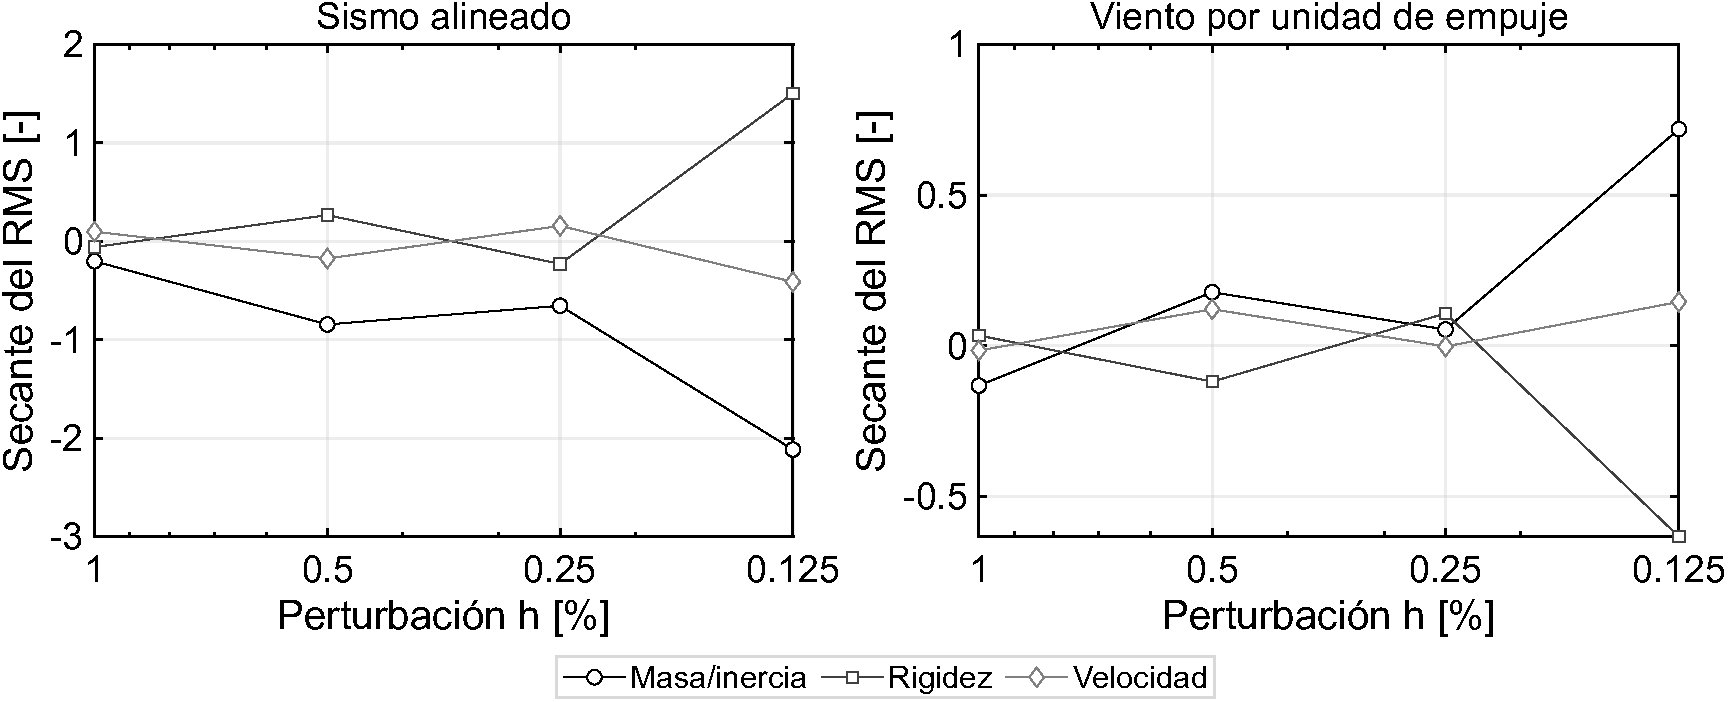
\includegraphics[width=.96\linewidth]{../entradas_reales_20261020/figures/refinamiento_sensibilidad.pdf}
\caption{Dependencia de las secantes del RMS de desplazamiento de góndola respecto de la perturbación mecánica. La ausencia de estabilización impide interpretar esas pendientes como derivadas locales resueltas.}\label{fig:refinamiento-temporal-reales}
\end{figure}
\begin{figure}[htbp]\centering
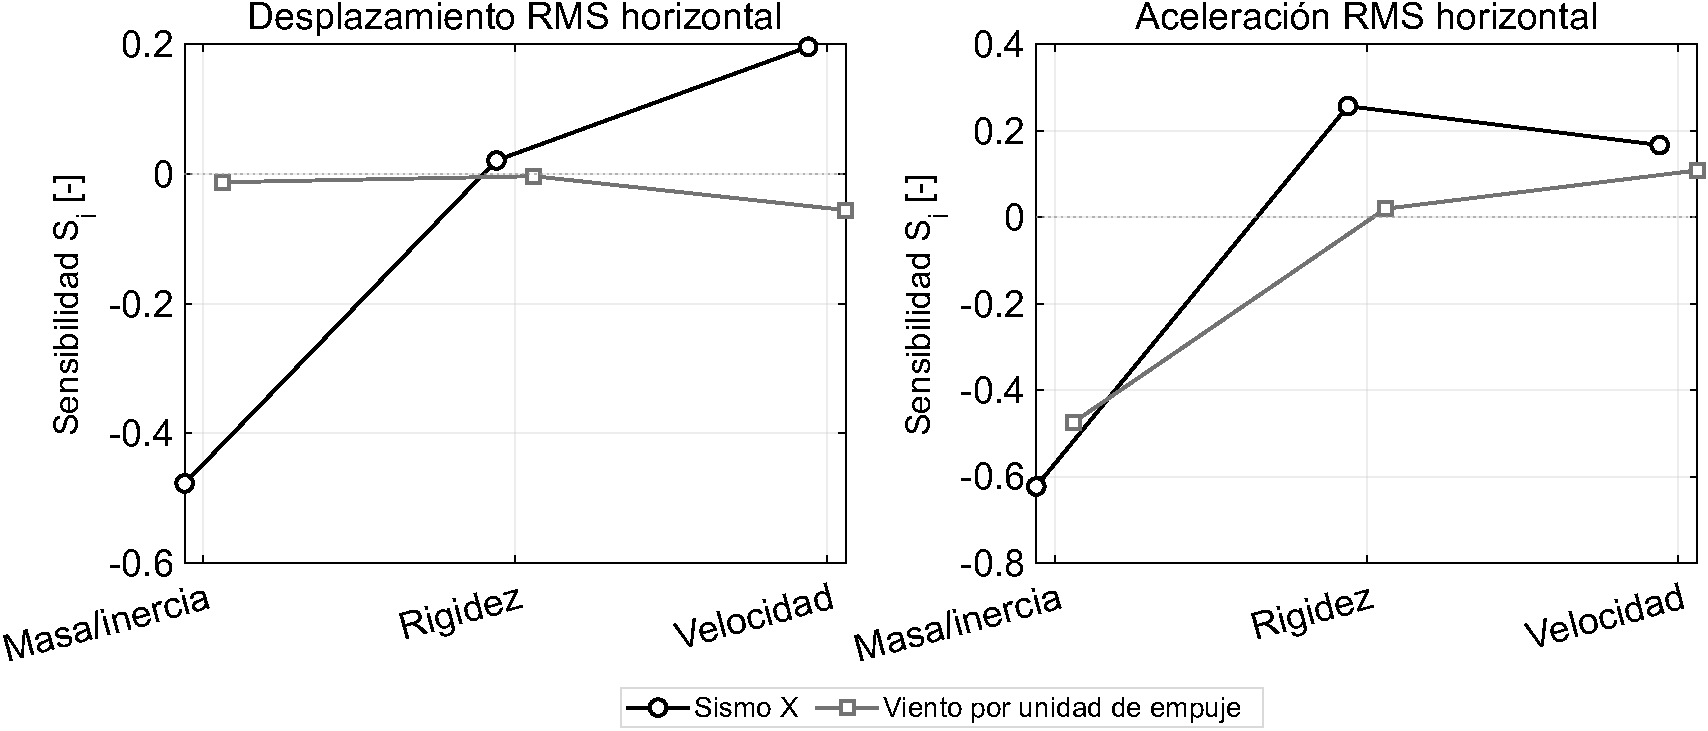
\includegraphics[width=.96\linewidth]{../entradas_reales_20261020/figures/sensibilidad_refinada.pdf}
\caption{Sensibilidades RMS de la góndola según la entrada. Con la Hessiana refinada, los símbolos llenos superan todos los filtros locales; los vacíos no se utilizan para establecer una clasificación definitiva. La respuesta de viento es por unidad de empuje medio.}\label{fig:sensibilidad-entradas-reales}
\end{figure}
\FloatBarrier

\subsection{Empuje libre, superposición y momento de llegada}
Para los mismos operadores lineales se obtiene exactamente
\begin{equation}
\boldsymbol q(t;\overline F,\tau)=\boldsymbol q_g(t-\tau)+
\frac{\overline F}{1\ \mathrm{kN}}\,\boldsymbol q_{w,1\mathrm{kN}}(t).
\end{equation}
La superposición se aplica a las historias, no a sus máximos separados. Se verificó además mediante una integración directa con la interfaz existente de sismo y fuerza externa completa durante 2 s. Esta identidad del problema implementado no afirma que la superposición sea exacta en un modelo aeroelástico no lineal.

Se define una escala de comparación
\begin{equation}
F_{\mathrm{ref}}=(1\ \mathrm{kN})\,
\frac{q_{H,\max}^g}{q_{H,\max}^{w,1\mathrm{kN}}}
=554.68\ \mathrm{kN},
\end{equation}
usando los primeros 39.98 s y llegada del sismo en cero. Esta escala iguala los máximos \emph{separados} de desplazamiento de góndola en esa ventana. No estima el empuje real, ni es un umbral de seguridad o de capacidad.

Se explora $\overline F/F_{\mathrm{ref}}$ entre 0 y 2 y 29 llegadas del sismo: $\tau=0,20,\ldots,540,559.98$ s. El último instante se ajusta al final de las muestras de viento, evitando extrapolación. El viento conserva su historia previa y cada máximo combinado usa la ventana $[\tau,\tau+39.98]$ s. No se inventa la cola sísmica después del registro ni se afirma que ese máximo sea el de los 600 s completos del escenario combinado. La franja de la figura es el mínimo y máximo de la rejilla temporal, no un intervalo de confianza.

Para $\overline F=F_{\mathrm{ref}}$, el cociente entre máximo combinado de desplazamiento y máximo sísmico varía entre 1.545 y 2.231 en las llegadas examinadas. Esa dependencia impide concluir que una de las entradas domina sin especificar empuje, dirección y ventana.
\begin{figure}[htbp]\centering
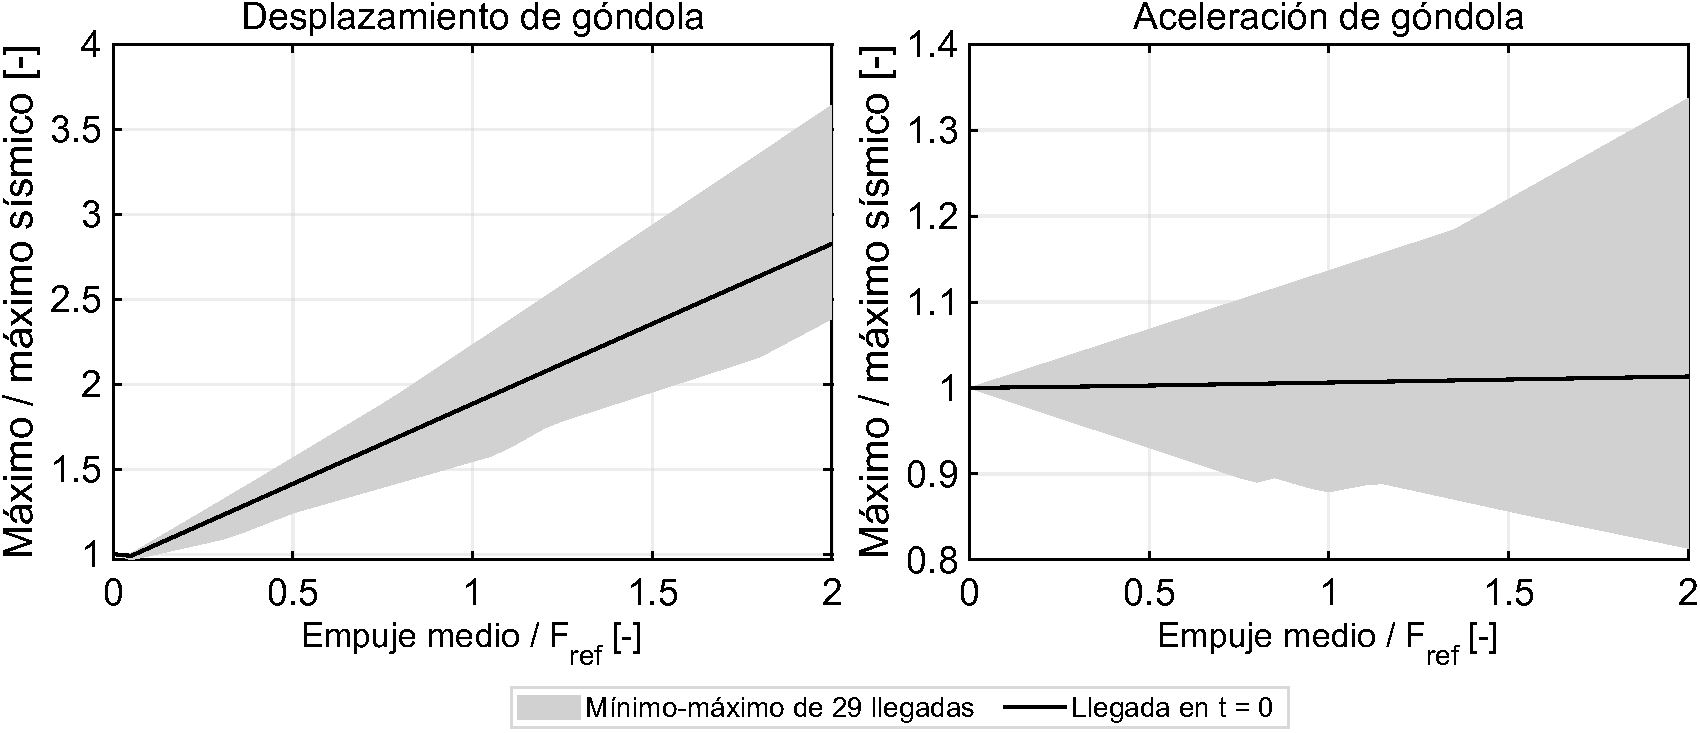
\includegraphics[width=.96\linewidth]{../entradas_reales_20261020/figures/combinacion_y_llegada.pdf}
\caption{Respuesta combinada parametrizada y efecto de la llegada sísmica. La línea usa $\tau=0$; la franja cubre las 29 llegadas. El empuje continúa como parámetro libre.}\label{fig:combinacion-reales}
\end{figure}
\begin{figure}[htbp]\centering
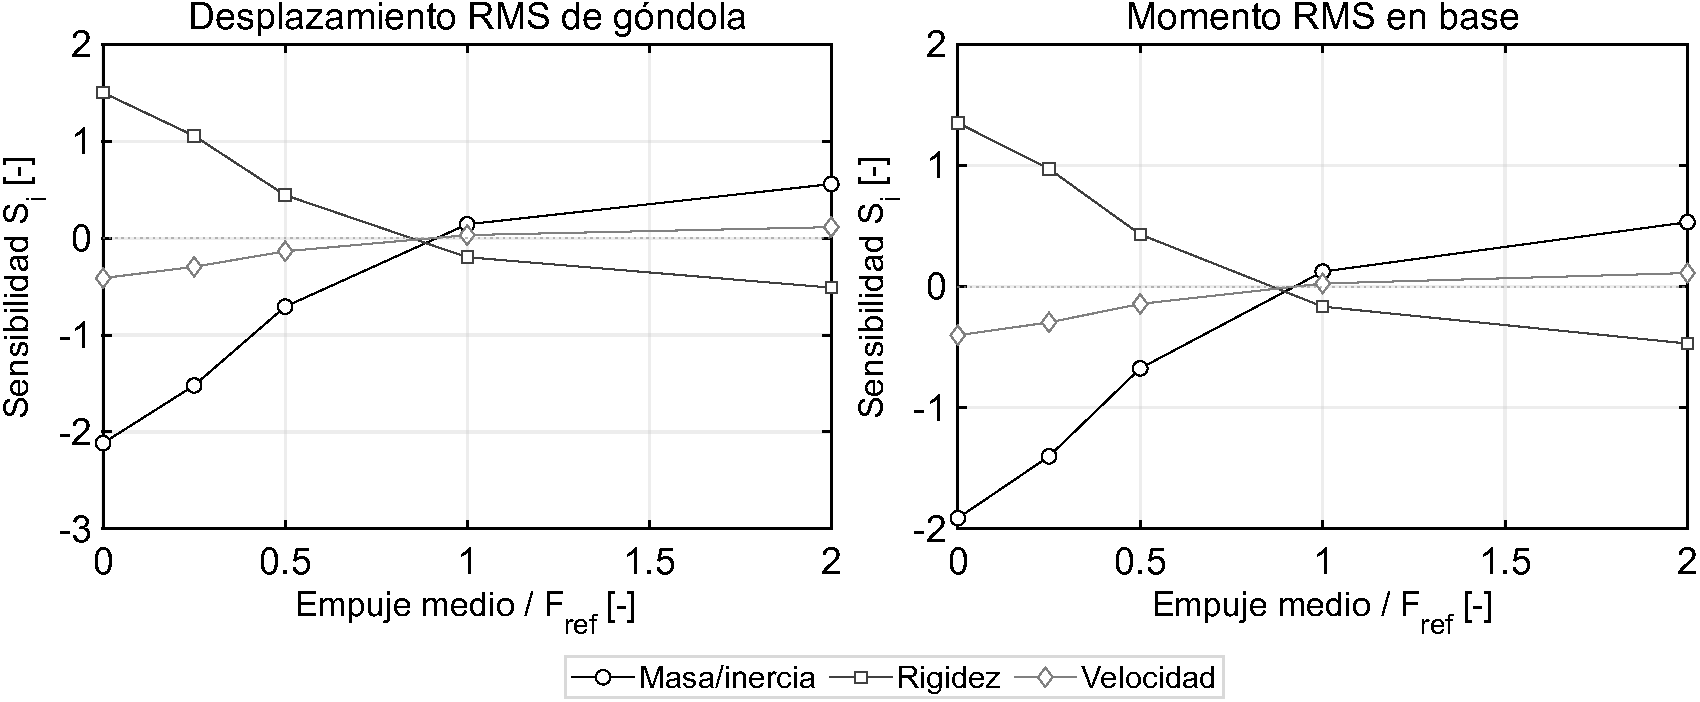
\includegraphics[width=.96\linewidth]{../entradas_reales_20261020/figures/sensibilidad_combinada.pdf}
\caption{Sensibilidades RMS de la respuesta combinada con llegada en cero. Los símbolos llenos indican compatibilidad de los pasos de diferenciación y de tiempo; ese control parcial no equivale a la aceptación completa de una sensibilidad Morris o local.}\label{fig:sensibilidad-combinada-reales}
\end{figure}
También se exportan sensibilidades respecto de la amplitud sísmica y del empuje medio. Para viento solo, toda respuesta homogénea no nula escala linealmente con $\overline F$, por lo que su sensibilidad normalizada es uno. En la combinación cambia la contribución relativa de cada entrada; en $\overline F=0$ la sensibilidad normalizada de ese parámetro se deja indefinida. Esto caracteriza dependencia respecto de amplitudes, no incertidumbre probabilística de los datos.
\begin{figure}[htbp]\centering
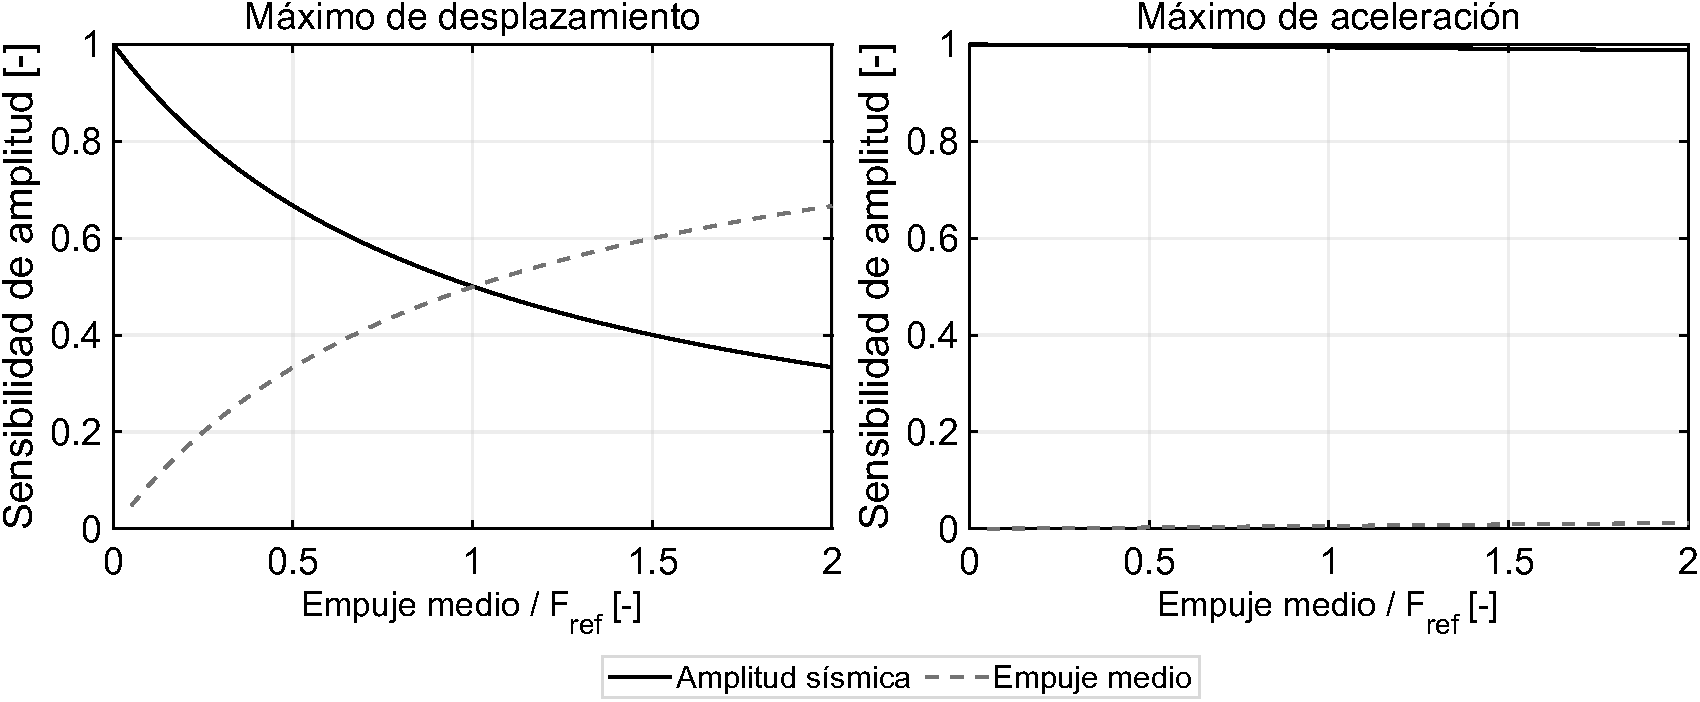
\includegraphics[width=.96\linewidth]{../entradas_reales_20261020/figures/sensibilidad_amplitudes.pdf}
\caption{Sensibilidad de los máximos de góndola respecto de un multiplicador de amplitud sísmica y del empuje medio. Se mantienen los mismos operadores, por lo que estos indicadores de amplitud no requieren diferenciar una rigidez reconstruida. No representan porcentajes probabilísticos de contribución.}\label{fig:amplitudes-reales}
\end{figure}
\FloatBarrier

\subsection{Verificación y conclusiones que se pueden sostener}
Se completaron 114 evaluaciones estructurales almacenadas; el residuo dinámico relativo máximo fue $8.30\times10^{-10}$. Las 175 fuentes congeladas de la campaña Morris conservan sus huellas. La recuperación por canales se contrastó con la rutina existente, con diferencias relativas menores que $5\times10^{-11}$. Para Arleta, los controles nominales de góndola entre 0.0025 y 0.00125 s muestran diferencias de máximo menores que 0.031\pct\ y diferencias temporales relativas menores que 0.315\pct. Estos controles no certifican todas las aceleraciones de puntas.

En una comprobación numérica independiente se varió únicamente el paso de la Hessiana de energía en una copia de diagnóstico, mediante las interfaces existentes de fuerza y tangente. La energía física y las 175 fuentes originales se conservaron. Se completaron 6 pruebas de diagnóstico y 1 no convergieron; los fallos se conservan en la tabla correspondiente. No se sustituyeron con este diagnóstico los operadores de los 114 casos comparativos. Para masa/inercia y máximo de góndola, las secantes con paso interno multiplicado por 20 fueron -0.5149 y -0.5155, al usar perturbaciones de 0.5 y 0.25\pct. Para masa/inercia y RMS de góndola, las secantes con paso interno multiplicado por 20 fueron -0.4793 y -0.4812, al usar perturbaciones de 0.5 y 0.25\pct. La dependencia del resultado con esta decisión numérica exige verificar la tangente antes de aceptar una clasificación mecánica temporal; el residuo de equilibrio pequeño no basta por sí solo.

El cierre alcanzado es una comparación con datos medidos, amplitudes trazables, orientación explícita y un empuje medio libre. Se distingue el efecto de los registros del efecto de los parámetros mecánicos; se conservan los indicadores que no superan los filtros. La clasificación modal de Morris no se traslada automáticamente a los máximos o RMS de una excitación particular.

Para convertir esta comparación en una predicción física de servicio hacen falta el empuje medio o una aerodinámica específica de la turbina, la validación de la transferencia espacial del viento y, para historias de operación, evolución de los operadores con el azimut. Permanecen pendientes la convergencia espacial en giro y la calibración experimental. La duración de los registros reales no convierte la instantánea congelada en una simulación de operación periódica.
% END REAL INPUTS 20261020



\section{Estabilidad, alcance y decisiones para continuar}
Las partes reales de los dieciséis representantes modales retornados por evaluación fueron negativas; la mayor observada fue $-0.01238$ s$^{-1}$. Bajo los operadores congelados, esto es compatible con decaimiento de esas perturbaciones modales seleccionadas. El espectro es parcial y no se calcula estabilidad periódica de Floquet: el dato no demuestra estabilidad de toda la turbina ni de todas las velocidades posibles. La sensibilidad de un centroide de crecimiento tampoco sustituye el examen de cada raíz.

La verificación espacial previa se realizó con rotor detenido, y la convergencia temporal corresponde al benchmark sísmico local anterior. No verifican automáticamente las sensibilidades globales en rotación. Esta etapa utiliza propiedades heredadas sin calibración experimental y tres factores elegidos; no estudia incertidumbre probabilística ni sensibilidad sísmica global.

Las siguientes decisiones científicas se pueden discutir con el asesor:
\begin{enumerate}
\item Obtener fuentes para rangos físicos y propiedades de palas, conexiones y apoyo. Esto permitiría pasar de escenarios a incertidumbre justificada.
\item Priorizar la convergencia espacial de las respuestas y sensibilidades con rotor en operación, conservando restricciones y seguimiento modal.
\item Ampliar la identificación masa--rigidez con otras respuestas y formas, partiendo de los contrastes ya comprobados en 10+11.
\item Definir si el alcance del artículo será sensibilidad a azimut fijo o si se requiere un estudio periódico adicional para afirmaciones de estabilidad.
\end{enumerate}
La comprobación de la rejilla y los contrastes finitos anteriores ya se ejecutaron. Los restantes puntos son propuestas científicas para acordar; no se han ejecutado campañas de refinamiento en operación ni estabilidad periódica.

\section{Guía breve para la reunión}
\paragraph{Apertura.} Se auditó y conservó el modelo existente, se implementó sensibilidad total con nuevo equilibrio y se pasó de derivadas locales a un cribado Morris sobre escenarios aprobados. La implementación conserva trazabilidad y rechaza resultados sin resolución suficiente.
\paragraph{Resultado principal.} La influencia depende del grupo: masa/inercia domina cuatro respuestas y velocidad domina 6+7 entre los tres factores. La frecuencia de 3 disminuye al aumentar giro; las de tres grupos superiores aumentan. Se usa la figura~\ref{fig:sentidos} para mostrar simultáneamente dirección y magnitud.
\paragraph{Mecanismo respaldado.} La participación nominal predominante de palas en 10 y 11 apoya la sensibilidad a sus propiedades. Las figuras~\ref{fig:dominio} y~\ref{fig:compensacion-rejilla} muestran la compensación parcial; los contrastes de la figura~\ref{fig:contrastes-interaccion} resuelven no aditividad masa--rigidez en 10+11. La separación exacta de contribuciones del giro sigue abierta.
\paragraph{Confianza y límite.} Catorce influencias y dos dispersiones superan los filtros. Los estimadores de influencia cambian menos de 1\pct\ al duplicar veinte a cuarenta trayectorias. Las figuras~\ref{fig:ruido} y~\ref{fig:dispersion} muestran por qué otros indicadores permanecen no resueltos. Esta evidencia es numérica y de azimut fijo.
\paragraph{Decisión a pedir.} Acordar cuál será la siguiente contribución: rangos físicos, convergencia espacial en operación, identificación con múltiples respuestas o extensión periódica. La elección debe estar ligada a la afirmación científica que se quiera sostener en el artículo y la tesis.

\appendix
\section{Valores de los catorce indicadores aceptados}
\begin{center}\small
\begin{tabular}{llrrr}
\toprule Factor & Grupo & $\mu_i$ & $\mu_i^*$ & $\sigma_i$ \\ \midrule
Masa/inercia & 3 & -0.11221 & 0.11221 & 0.01052 \\
Masa/inercia & 4+5 & -0.11335 & 0.11335 & 0.00670 \\
Masa/inercia & 6+7 & -0.06161 & 0.06161 & 0.00398 \\
Masa/inercia & 8+9 & -0.08546 & 0.08546 & 0.00495 \\
Masa/inercia & 10+11 & -0.07653 & 0.07653 & 0.00445 \\
Rigidez & 3 & +0.07695 & 0.07695 & 0.00652 \\
Rigidez & 4+5 & +0.07886 & 0.07886 & 0.00368 \\
Rigidez & 6+7 & +0.04866 & 0.04866 & 0.00235 \\
Rigidez & 8+9 & +0.07296 & 0.07296 & 0.00291 \\
Rigidez & 10+11 & +0.07172 & 0.07172 & 0.00283 \\
Velocidad & 3 & -0.05952 & 0.05952 & 0.00726 \\
Velocidad & 6+7 & +0.06923 & 0.06923 & 0.00202 \\
Velocidad & 8+9 & +0.02295 & 0.02295 & 0.00155 \\
Velocidad & 10+11 & +0.03678 & 0.03678 & 0.00173 \\

\bottomrule
\end{tabular}
\end{center}
La aceptación de $\mu_i^*$ en esta tabla no implica aceptación de $\sigma_i$ en todas sus filas. Los controles de dispersión se evalúan por separado. Los números se redondean para lectura; las tablas CSV y MAT conservan mayor precisión.

Las figuras históricas se exportaron desde Tecplot y se incluyen como PDF externos. Los datos, macros y paquetes nativos permanecen en su biblioteca. Las figuras nuevas y las adaptaciones para proyección se exportaron desde MATLAB con autorización del autor ante la licencia Tecplot vencida. Las fuentes originales se conservan en morris\_estimators.csv, morris\_sweeps.csv, morris\_vertices.csv, report\_data.json y modal\_energy\_evidence.csv. La comprobación adicional usa grid\_responses.csv y sus tablas de contrastes. No se reemplazaron casos fallidos; los nueve casos nuevos se registran en una campaña separada.

\begin{thebibliography}{9}
\bibitem{morris1991} M. D. Morris. Factorial Sampling Plans for Preliminary Computational Experiments. \emph{Technometrics}, 33(2), 161--174, 1991. \href{https://doi.org/10.1080/00401706.1991.10484804}{doi:10.1080/00401706.1991.10484804}.
\bibitem{campolongo2007} F. Campolongo, J. Cariboni y A. Saltelli. An effective screening design for sensitivity analysis of large models. \emph{Environmental Modelling \& Software}, 22(10), 1509--1518, 2007. \href{https://doi.org/10.1016/j.envsoft.2006.10.004}{doi:10.1016/j.envsoft.2006.10.004}.

\bibitem{wang2026inputs} W. Wang, H. Diao, H. Ma, X. Gao, B. Ji y Z. Zhang. Research on the Dynamic Response of Hybrid Tower Wind Turbines Under Combined Earthquake--Wind Multi-Hazard Conditions. \emph{Journal of Earthquake Engineering}, 2026. \href{https://doi.org/10.1080/13632469.2026.2671807}{doi:10.1080/13632469.2026.2671807}.
\bibitem{diao2026data} H. Diao. Data of Research on the Dynamic Response of Hybrid Tower Wind Turbines under Combined Earthquake--Wind Multi-Hazard Conditions. Zenodo, versión consultada 19347779, 2026. \href{https://doi.org/10.5281/zenodo.19347779}{doi:10.5281/zenodo.19347779}.
\bibitem{meng2020} J. Meng, K. Dai, Z. Zhao, Z. Mao, A. Camara, S. Zhang y Z. Mei. Study on the aerodynamic damping for the seismic analysis of wind turbines in operation. \emph{Renewable Energy}, 159, 1224--1242, 2020. \href{https://doi.org/10.1016/j.renene.2020.05.181}{doi:10.1016/j.renene.2020.05.181}.
\bibitem{turello2023inputs} D. F. Turello, M. S. Maza, S. Preidikman, F. G. Flores y F. Pinto. Interacción suelo-estructura no-lineal en el modelado de torres eólicas de eje horizontal ante carga sísmica. \emph{Mecánica Computacional}, XL, 639--650, 2023. \url{https://cimec.org.ar/ojs/index.php/mc/article/view/6595}.
\bibitem{dtu2021inputs} K. S. Hansen, N. Vasiljevic y S. A. Sørensen. Turbulence and turbine measurements from the NM92 turbine. DTU Data, 2021. \href{https://doi.org/10.11583/DTU.16743739}{doi:10.11583/DTU.16743739}. Datos CC BY 4.0.
\bibitem{openseesinputs} OpenSees. Repositorio oficial: registros PEER procesados en \texttt{EXAMPLES/ExampleScripts} y \texttt{Workshops/SimWorkshop/SmallMP/GM}. \url{https://github.com/OpenSees/OpenSees}. La revisión exacta, rutas y SHA-256 se conservan en el catálogo de entradas del proyecto.

\end{thebibliography}
\end{document}
